%!TEX root = ../Master_template.tex
\chapter{Experiments}
\label{chapter:experiments}

In this chapter, we describe the datasets used for all experiments in both time series forecasting and classification (see Section~\ref{sec:datasets}). The experimental setup—including the models, their parameters, hyperparameter configurations, and the tuning of augmentation methods for both forecasting and classification—is detailed in Section~\ref{sec:experimental_setup}. Section~\ref{sec:main_results} presents the main results for long-term and short-term forecasting, as well as univariate and multivariate time series classification. Finally, Section~\ref{sec:ablation} provides various ablation studies related to our proposed methods, covering both forecasting and classification tasks.

\section{Datasets} \label{sec:datasets}

\subsection*{Time Series Forecasting} \label{subsec:dataset-tsf}


We utilize seven benchmark datasets for long-term time series forecasting and four datasets for short-term forecasting tasks. A summary of these datasets is provided in Table~\ref{tab:datasets}. Datasets ranging from ETTh1 to Influenza-like Illness (ILI) are employed for long-term forecasting, while all Caltrans Performance Measurement System (PeMS) datasets are used for short-term forecasting. These datasets span diverse domains and dimensionalities, enabling a comprehensive evaluation of the effectiveness and generalizability of our proposed augmentation method.
The Electricity Transformer Temperature (ETT) datasets~\cite{zhou2021informerefficienttransformerlong} consist of seven variables recorded from electricity transformers, covering the period from July 2016 to July 2018. The ETT datasets are divided into four subsets: ETTh1 and ETTh2, recorded at hourly intervals, and ETTm1 and ETTm2, recorded every 15 minutes.
The Exchange dataset~\cite{wu2022autoformerdecompositiontransformersautocorrelation} contains daily exchange rates from eight countries between 1990 and 2016. The Weather dataset~\cite{wu2022autoformerdecompositiontransformersautocorrelation} includes 21 meteorological variables measured every 10 minutes at the Max Planck Institute for Biogeochemistry Weather Station throughout 2020. We note that experiments were not conducted on the Electricity Consuming Load (ECL), Traffic, Solar-Energy~\cite{lai2018modelinglongshorttermtemporal} due to their substantially higher computational demands (i.e., increased GPU memory and extended training times), which exceeded the available resources for this study.
For short-term forecasting, we utilize the PeMS datasets, which consist of publicly available traffic sensor data collected across California at 5-minute intervals. We adopt four subsets—PeMS03, PeMS04, PeMS07, and PeMS08—as standardized in the SCINet framework~\cite{liu2022scinettimeseriesmodeling}. Table~\ref{tab:datasets} summarizes the input dimensionality, prediction lengths, and dataset sizes for training, validation, and test splits.

\begin{table}[h!]
\vspace{0.5cm}
\centering
\scriptsize
\renewcommand{\arraystretch}{1.2}
\setlength{\tabcolsep}{8pt}
\begin{tabular}{lcccc}
\toprule
\textbf{Dataset} & \textbf{Dim.} & \textbf{Prediction Length} & \textbf{Dataset Size} & \textbf{Information} \\
\midrule
ETTh1 & 7 & \{96, 192, 336, 720\} & (8545, 2881, 2881) & Electricity (Hourly) \\
ETTh2 & 7 & \{96, 192, 336, 720\} & (8545, 2881, 2881) & Electricity (Hourly) \\
ETTm1 & 7 & \{96, 192, 336, 720\} & (34465, 11521, 11521) & Electricity (15min) \\
ETTm2 & 7 & \{96, 192, 336, 720\} & (34465, 11521, 11521) & Electricity (15min) \\
Exchange & 8 & \{96, 192, 336, 720\} & (5120, 665, 1422) & Economy (Daily) \\
Weather & 21 & \{96, 192, 336, 720\} & (36792, 5271, 10540) & Weather (10min) \\
ILI & 7 & \{24, 36, 48, 60\} & (629, 98, 194) & Illness (Weekly) \\
PeMS03 & 358 & \{12, 24, 36, 48\} & (15617, 5135, 5135) & Transportation (5min) \\
PeMS04 & 307 & \{12, 24, 36, 48\} & (10172, 3375, 3375) & Transportation (5min) \\
PeMS07 & 883 & \{12, 24, 36, 48\} & (16911, 5622, 5622) & Transportation (5min) \\
PeMS08 & 170 & \{12, 24, 36, 48\} & (10690, 3548, 3548) & Transportation (5min) \\
\bottomrule
\end{tabular}
\caption{Summary of the datasets used in time series forecasting experiments. The table includes input dimensionality (number of channels), prediction lengths, and dataset sizes for training, validation, and test splits. The datasets span a variety of domains (e.g., electricity, weather, transportation, health) and temporal granularities, supporting both long-term and short-term forecasting tasks~\cite{liu2024itransformerinvertedtransformerseffective}.}
\label{tab:datasets}
\end{table}





\subsection*{Time Series Classification} \label{subsec:datasets-tsc}


We utilize the widely used UCR~\cite{UCRArchive2018} and UEA~\cite{bagnall2018ueamultivariatetimeseries} repositories to evaluate our methodology in univariate and multivariate time series classification tasks.

The UCR archive is extensively utilized within the time series research community and contains solely univariate datasets, each featuring a singular time-dependent variable (i.e., one channel). It is divided into different categories: Device, ECG, Image, Motion, Sensor, Spectrograph, Simulated, and others~\cite{UCRArchive2018}. For our assessment, we chose a varied subset of 128 datasets by incorporating representative samples from different categories. The datasets exhibit variation in training/test sizes, sequence lengths, and output class numbers, making the evaluation extensive and comprehensive. Table~\ref{tab:tsc_datasets} shows the main characteristics of the chosen UCR datasets used in our experiments.




\begin{table}[h!]
\centering
\vspace{0.2cm}
\begin{adjustbox}{max width=\textwidth}
\begin{tabular}{llcccc}
\toprule
\textbf{Type} & \textbf{Dataset} & \textbf{Train Size} & \textbf{Test Size} & \textbf{Length} & \textbf{No. of Classes} \\
\midrule
\multirow{3}{*}{\textbf{Device}} 
& ACSF1 & 100 & 100 & 1460 & 10 \\
& HouseTwenty & 34 & 101 & 3000 & 2 \\
& ScreenType & 375 & 375 & 720 & 3 \\
\midrule
\multirow{3}{*}{\textbf{ECG}} 
& ECG5000 & 500 & 4500 & 140 & 5 \\
& ECG200 & 100 & 100 & 96 & 2 \\
& ECGFiveDays & 23 & 861 & 136 & 2 \\
\midrule
\multirow{7}{*}{\textbf{Image}} 
& Adiac & 390 & 391 & 176 & 37  \\
& FaceFour & 24 & 88 & 350 & 4  \\
& FaceAll & 560 & 1690 & 131 & 14 \\
& HandOutlines & 1000 & 370 & 2709 & 2 \\
& MiddlePhalanxTW & 399 & 154 & 80 & 6 \\
& PhalangesOutlinesCorrect & 1800 & 858 & 80 & 2 \\
& ShapesAll & 600 & 600 & 512 & 60 \\
\midrule
\multirow{3}{*}{\textbf{Motion}} 
& Haptics & 155 & 308 & 1092 & 5 \\
& WormsTwoClass & 181 & 77 & 900 & 2  \\
& InlineSkate & 100 & 550 & 1882 & 7  \\
\midrule
\multirow{7}{*}{\textbf{Sensor}} 
& Car & 60 & 60 & 577 & 4 \\
& Earthquakes & 322 & 139 & 512 & 2 \\
& FordA & 3601 & 1320 & 500 & 2  \\
& FordB & 3636 & 810 & 500 & 2  \\
& ItalyPowerDemand & 67 & 1029 & 24 & 2  \\
& Lightning2 & 60 & 61 & 637 & 2  \\
& StarLightCurves & 1000 & 8236 & 1024 & 3  \\
\midrule
\multirow{5}{*}{\textbf{Spectro}} 
& Beef & 30 & 30 & 470 & 5  \\
& EthanolLevel & 504 & 500 & 1751 & 4  \\
& Wine & 57 & 54 & 234 & 2  \\
& Meat & 60 & 60 & 448 & 3 \\
& OliveOil & 30 & 30 & 570 & 4  \\
\midrule
\multirow{2}{*}{\textbf{Simulated \& Audio}} 
& ChlorineConcentration & 467 & 3840 & 166 & 3 \\
& Phoneme & 214 & 1896 & 1024 & 39 \\
\bottomrule
\end{tabular}
\end{adjustbox}
\caption{Summary of selected UCR univariate time series classification datasets used in our experiments. The table includes dataset category, name, training and test set sizes, input sequence lengths, and number of output classes~\cite{UCRArchive2018}.}
\label{tab:tsc_datasets}
\end{table}

In contrast, the UEA archive pertains to multivariate time series classification tasks. The datasets consist of various channels with input features varying from 2 to 1345~\cite{bagnall2018ueamultivariatetimeseries}. We selected 10 datasets from the 30 in the UEA archive representing diverse characteristics, covering multiple application domains and varying dimensionality. Table~\ref{tab:tsc_multivariate} provides detailed information about the chosen UEA datasets, including their sizes, sequence lengths, dimensionality, and number of output classes.




\begin{table}[h!]
\centering
\begin{adjustbox}{max width=\textwidth}
\begin{tabular}{lccccc}
\toprule
\textbf{Dataset} & \textbf{Train Size} & \textbf{Test Size} & \textbf{Dimensions} & \textbf{Length} & \textbf{No. of Classes} \\
\midrule
AtrialFibrillation & 15 & 15 & 2 & 640 & 3 \\
Cricket & 108 & 72 & 6 & 1197 & 12 \\
DuckDuckGeese & 60 & 40 & 1345 & 270 & 5 \\
ERing & 30 & 30 & 4 & 65 & 6 \\
EthanolConcentration & 261 & 263 & 3 & 1751 & 4 \\
LSST & 2459 & 2466 & 6 & 36 & 14 \\
Libras & 180 & 180 & 2 & 45 & 15 \\
FaceDetection & 5890 & 3524 & 144 & 62 & 2 \\
FingerMovements & 316 & 100 & 28 & 50 & 2 \\
MotorImagery & 278 & 100 & 64 & 3000 & 2 \\
\bottomrule
\end{tabular}
\end{adjustbox}
\caption{Characteristics of the multivariate time series classification datasets selected from the UEA archive. These datasets span a wide range of application domains and vary significantly in input dimensionality, sequence length, and number of classes, offering a robust benchmark for evaluating model performance on multivariate data~\cite{bagnall2018ueamultivariatetimeseries}.}
\label{tab:tsc_multivariate}
\end{table}

The UCR and UEA repositories are standard benchmarks in time series classification literature and are frequently employed in comparative studies~\cite{UCRArchive2018, bagnall2018ueamultivariatetimeseries}. Our evaluation achieves broad applicability through experimentation on datasets from both repositories and ensures comparable results. 


\section{Experimental Setup} \label{sec:experimental_setup}

\subsection*{Time Series Forecasting} \label{subsec:experimental_setup-tsf}


We utilize five distinct models for long-term forecasting tasks, encompassing linear architectures with multi-layer perceptrons (MLPs) and Transformer-based frameworks. This selection allows an in-depth evaluation of the effectiveness of our augmentation method across various modeling frameworks.

PatchTST~\cite{nie2023timeseriesworth64} is an efficient Transformer-based model that partitions time series into segments, treating these segments as input tokens for the Transformer. In addition, PatchTST employs a channel-independent architecture, facilitating the efficient modeling of temporal dependencies across distinct features~\cite{nie2023timeseriesworth64}.

DLinear~\cite{zeng2022transformerseffectivetimeseries} demonstrates a completely linear methodology, wherein the authors illustrated that even basic, single-layer linear models could surpass some Transformer-based architectures in long-term forecasting tasks.

TSMixer~\cite{chen2023tsmixerallmlparchitecturetime} is a model formed by stacked multi-layer perceptrons (MLPs). It successfully integrates information across temporal and feature dimensions via MLP operations, providing a highly scalable and straightforward alternative to traditional sequence models~\cite{chen2023tsmixerallmlparchitecturetime}.

Time-series Dense Encoder (TiDE)~\cite{das2024longtermforecastingtidetimeseries} follows an encoder-decoder design based entirely on MLPs. It can model non-linear dependencies and effectively handle covariates, making it particularly suitable for more complex forecasting settings~\cite{das2024longtermforecastingtidetimeseries}.


LightTS~\cite{zhang2022morefastmultivariatetime} is a lightweight deep learning model combining MLP-based processing with two down-sampling strategies: interval and continuous. This design reduces computational complexity while preserving essential temporal information~\cite{zhang2022morefastmultivariatetime}.


Applying these models guarantees that our experimental evaluation covers a broad spectrum of architectures with various modeling assumptions and complexities. This enables a comprehensive evaluation of the robustness and effectiveness of our proposed augmentation method.


Ultimately, while our emphasis is on linear, MLP-based, and Transformer-based models, we will address the prospective application of our methodology to graph neural networks (GNNs) and recurrent neural networks (RNNs) in future work (see Section~\ref{sec:future}).

The input sequence lengths are chosen according to the optimal configurations reported in the original studies, as our aim is to evaluate augmentation techniques under optimal model conditions fairly. During training, we configured the number of epochs to 20 (except that it is less than 20 in the original configuration), employing early stopping with the patience of 10 epochs and saving the model weights, which resulted in the lowest validation loss. Despite certain original studies indicating training for 100 epochs or more, we limit the training to fewer due to computational constraints. However, this change only results in minor inconsistencies relative to the initial findings and does not affect the overall conclusions.

Learning rate schedulers are chosen according to the recommendations of the original papers when available or alternatively based on our empirical evaluation to ensure stable convergence. Learning rates are calibrated either based on the initial configurations or through validation-driven adjustments.

The input sequence lengths are set as follows:


\begin{itemize}
    \item For DLinear and PatchTST, the input sequence length is 336.
    \item For TiDE and LightTS, it is 720.
    \item For TSMixer, the input sequence length is 512.
\end{itemize}

For specific datasets, such as ILI, the sequence length is reduced to 104, following the guidelines from the corresponding papers and confirmed by our own evaluation. This adjustment is necessary because these datasets contain relatively few temporal points, making longer input sequences impractical~\cite{zeng2022transformerseffectivetimeseries, nie2023timeseriesworth64}.

By carefully adjusting input lengths, learning rates, and schedulers by best practices, we ensure that our augmentation method is assessed under fair and competitive conditions across all baseline models.



We optimized the hyperparameters of several augmentation techniques, including FreqAdd, FreqPool, Upsample, Frequency Masking (FreqMask), Frequency Mixing (FreqMix), Dominant Shuffle, and our proposed method, Temporal Patch Shuffle (TPS), on the ETTh1, ETTh2, ETTm1, and ETTm2 datasets using the TSMixer model. Due to computational constraints, we did not perform hyperparameter tuning for methods such as weighted Dynamic Time Warping Barycentric Averaging (wDBA), Moving Block Bootstrapping (MBB), RobustTAD,  Spectral and Time Augmentation (STAug), wavelet masking (WaveMask), and wavelet mixing (WaveMix).
Table~\ref{tab:aug_params} outlines the key hyperparameters associated with each augmentation method. RobustTAD-m/p indicates that the RobustTAD method has been applied either to the magnitude or the phase component. For our method TPS, we evaluated 25 distinct configurations (see Table~\ref{tab:tps_parameters_split1}). Each configuration was run five times, and the optimal setting was selected based on the validation loss, while also considering the standard deviation to ensure robustness.

\begin{table}[h!]
\centering
\begin{tabular}{@{}ll@{}}
\toprule
\textbf{Method} & \textbf{Parameters} \\
\midrule
wDBA              & weighting, DTW constraints \\
MBB               & block size, STL period \\
RobustTAD-m/p     & perturbation rate, number of segments, segment length \\
FreqAdd           & perturbation rate \\
FreqPool          & pool size \\
Upsample          & subsequence length rate \\
STAug             & mixup rate \\
FreqMask          & masking rate \\
FreqMix           & mixing rate \\
WaveMix \& WaveMask      & wavelet type, decomposition level, sampling rate \\
Dominant Shuffle  & shuffle rate \\
TPS               & patch length, stride, shuffle rate \\
\bottomrule
\end{tabular}
\caption{Hyperparameters used for each time series forecasting augmentation method.}

\label{tab:aug_params}
\end{table}



\begin{table}[h!]
\centering
\begin{minipage}[t]{0.48\linewidth}
\centering
\begin{tabular}{@{}cccc@{}}
\toprule
\# & $p$ & $s$ & $\alpha$ \\
\midrule
1  & 16  & 5   & 0.8 \\
2  & 16  & 12  & 0.9 \\
3  & 16  & 1   & 1.0 \\
4  & 32  & 5   & 1.0 \\
5  & 32  & 8   & 0.9 \\
6  & 32  & 8   & 1.0 \\
7  & 32  & 12  & 0.7 \\
8  & 32  & 16  & 1.0 \\
9  & 64  & 2   & 1.0 \\
10 & 72  & 24  & 1.0 \\
11 & 96  & 2   & 1.0 \\
12 & 96  & 16  & 0.7 \\
13 & 96  & 32  & 0.9 \\
\bottomrule
\end{tabular}
\end{minipage}
\hfill
\begin{minipage}[t]{0.48\linewidth}
\centering
\begin{tabular}{@{}cccc@{}}
\toprule
\# & $p$ & $s$ & $\alpha$ \\
\midrule
14 & 96  & 96  & 1.0 \\
15 & 120 & 12  & 0.9 \\
16 & 120 & 12  & 1.0 \\
17 & 120 & 24  & 1.0 \\
18 & 120 & 36  & 1.0 \\
19 & 120 & 1   & 1.0 \\
20 & 168 & 24  & 0.8 \\
21 & 192 & 12  & 0.8 \\
22 & 200 & 24  & 1.0 \\
23 & 220 & 8   & 1.0 \\
24 & 240 & 24  & 0.8 \\
25 & 240 & 24  & 1.0 \\
\bottomrule
\end{tabular}
\end{minipage}
\caption{Hyperparameter configurations used for TPS. Each configuration is defined by patch length ($p$), stride ($s$), and shuffle rate ($\alpha$).}
\label{tab:tps_parameters_split1}
\end{table}



For other models and datasets, we used the hyperparameters provided in the respective original papers. For our method, we experimented with only a small subset of configurations. Although the original papers did not state it explicitly, we observed during reproduction that hyperparameters were selected based on test loss. Therefore, fully calibrated results for the most relevant augmentation methods using TSMixer are reported in Table~\ref{tb: ts1}.


For short-term forecasting, we exclusively employed the PatchTST model, which is computationally expensive due to the large number of input channels. For this model, we adopted hyperparameters from the original papers for each augmentation method, but for our method, we tested 8–10 configurations and selected the best one based on validation loss.

Given our computational limitations, all experiments were conducted fairly and consistently, laying the groundwork for further improvements in future work.


\subsection*{Time Series Classification} \label{subsec:experimental_setup-tsc}



We utilized models from the RandOm Convolutional KErnel Transform (ROCKET) family~\cite{Dempster_2020}, specifically MINImally RandOm Convolutional KErnel Transform (MiniRocket)\cite{Dempster_2021} for univariate datasets and MultiRocket\cite{tan2022multirocketmultiplepoolingoperators} for multivariate time series classification.

ROCKET transforms input time series using 10,000 randomly generated convolutional kernels. Each kernel produces two features via max pooling and PPV (proportion of positive values) pooling, resulting in 20,000 features per input. These transformed features are then passed to a linear classifier, such as ridge regression or logistic regression. The kernels are randomly parameterized in terms of length, weights, bias, dilation, and padding~\cite{Dempster_2020}.

MiniRocket improves upon ROCKET by employing a fixed, deterministic set of kernels, significantly reducing computational cost and achieving up to a 75x speed-up on large datasets~\cite{Dempster_2020, Dempster_2021}.

MultiRocket further extends MiniRocket by introducing two key enhancements: it applies a first-order difference transform to the input and incorporates three additional pooling operators per kernel~\cite{tan2022multirocketmultiplepoolingoperators}. In our experiments, we used MultiRocket for the multivariate classification setting.

Applying these models provided initial insights into how TPS integrates with kernel-based time series approaches. Due to time and computational constraints, we did not implement other models such as InceptionTime~\cite{Ismail_Fawaz_2020}; this is discussed further in Section~\ref{sec:future}.


We used RidgeClassifier for MiniRocket and Logistic Regression for MultiRocket, running each model for five iterations. All parameters, including the number of features, number of kernels, and other settings, strictly follow those reported in the original papers.

We have used the original parameters from the papers for the augmentation methods~\cite{10.1371/journal.pone.0254841}. The methods and their corresponding parameters are given in the Table~\ref{tab:tsc_aug_params}.

\begin{table}[h!]
\centering
\begin{tabular}{@{}ll@{}}
\toprule
\textbf{Method} & \textbf{Parameters} \\
\midrule
Jittering        & standard deviation \\
Scaling          & standard deviation \\
Permutation      & window size, number of permutations \\
Mag. Warping  & standard deviation, number of knots \\
Time Warping  & standard deviation, number of knots \\
Window Slice  & window size \\
Window Warping  & window size, warping amount \\
Rotation         & – \\
SPAWNER          & standard deviation, DTW constraints \\
RGW, RGWs        & DTW constraints \\
DGW, DGWs        & DTW constraints \\
wDBA             & weighting, DTW constraints \\
TPS, TIPS              & patch length, stride, shuffle rate \\
\bottomrule
\end{tabular}
\caption{Parameters used for each time series classification augmentation method.}
\label{tab:tsc_aug_params}
\end{table}

For both TPS method and Temporal Index Patch Shuffle (TIPS), we split each dataset into 80\% training and 20\% validation sets. Hyperparameters were selected based on the configuration that yielded the highest validation accuracy. In cases where multiple configurations achieved the same accuracy, one was randomly chosen for final training on the whole training set and evaluation on the test set. It is essential to note that the test data was already provided as a separate file for each dataset. The hyperparameter configurations for TPS and TIPS are presented in Table~\ref{tab:tps_parameters_split}. In total, we evaluated 36 different randomly sampled hyperparameter combinations.

\begin{table}[h!]
\centering
\begin{minipage}[t]{0.48\linewidth}
\centering
\begin{tabular}{@{}cccc@{}}
\toprule
\# & $p$ & $s$ & $\alpha$ \\
\midrule
1  & 2    & 1   & 0.4 \\
2  & 4    & 4   & 0.6 \\
3  & 6    & 4   & 1.0 \\
4  & 8    & 4   & 1.0 \\
5  & 12   & 96  & 0.8 \\
6  & 24   & 36  & 0.8 \\
7  & 32   & 1   & 0.6 \\
8  & 48   & 36  & 0.9 \\
9  & 64   & 2   & 0.6 \\
10 & 64   & 24  & 0.8 \\
11 & 64   & 24  & 1.0 \\
12 & 72   & 2   & 0.4 \\
13 & 96   & 8   & 0.8 \\
14 & 96   & 96  & 1.0 \\
15 & 96   & 96  & 0.6 \\
16 & 120  & 1   & 1.0 \\
17 & 120  & 1   & 0.7 \\
18 & 120  & 48  & 0.8 \\
\bottomrule
\end{tabular}
\end{minipage}
\hfill
\begin{minipage}[t]{0.48\linewidth}
\centering
\begin{tabular}{@{}cccc@{}}
\toprule
\# & $p$ & $s$ & $\alpha$ \\
\midrule
19 & 120  & 1   & 0.2 \\
20 & 148  & 24  & 1.0 \\
21 & 148  & 96  & 1.0 \\
22 & 148  & 48  & 1.0 \\
23 & 148  & 48  & 1.0 \\
24 & 152  & 96  & 1.0 \\
25 & 180  & 12  & 0.8 \\
26 & 180  & 24  & 0.8 \\
27 & 180  & 12  & 0.5 \\
28 & 240  & 1   & 0.8 \\
29 & 240  & 1   & 0.4 \\
30 & 240  & 1   & 0.2 \\
31 & 240  & 96  & 1.0 \\
32 & 280  & 8   & 0.1 \\
33 & 360  & 1   & 0.1 \\
34 & 480  & 1   & 0.7 \\
35 & 900  & 1   & 0.8 \\
36 & 1220 & 48  & 0.1 \\
\bottomrule
\end{tabular}
\end{minipage}
\caption{Explored hyperparameter configurations for the TPS and TIPS methods in time series classification. Each configuration is defined by a patch length ($p$), stride ($s$), and shuffle rate ($\alpha$). A total of 36 configurations were randomly sampled and evaluated based on validation accuracy.}
\label{tab:tps_parameters_split}
\end{table}



\section{Main Results} \label{sec:main_results}

The main results are presented and discussed in this section. For time series forecasting, we report the average performance of each model across all datasets and prediction lengths, as well as the average across prediction lengths for each dataset and model. Results are presented separately for long-term and short-term forecasting (see Section~\ref{subsec:main_results-tsf}). For time series classification, we present the main results for both univariate and multivariate settings using two different models (see Section~\ref{subsec:main_results-tsc}).

\subsection{Results for Time Series Forecasting} \label{subsec:main_results-tsf}


Before presenting the results for each dataset, we first provide the overall average performance across all datasets and prediction lengths, reported in terms of Mean Squared Error (MSE) and Mean Absolute Error (MAE) for each model and augmentation method in Table~\ref{tb:avg_model_results}. The values are averaged over all 28 runs (i.e., 4 prediction lengths × 7 datasets).
In this table, RobustTAD-m/p refers to the best result selected from RobustTAD implementations applied to either the magnitude or phase components. Freq-MixMax and Wave-MixMax denote the best outcomes obtained among FreqMax/FreqMix and WaveMask/WaveMix versions, respectively. The best results are highlighted in \textbf{green and bold}, and the second-best in blue. The \textbf{\#Wins} row indicates how many times TPS achieved the best result across the 28 settings. The \textbf{Improvement} column shows the relative percentage gain of TPS over the second-best augmentation method. It is evident that TPS achieved improvements of \textbf{2.98\%}, \textbf{5.83\%}, \textbf{3.16\%}, \textbf{2.26\%}, and \textbf{10.90\%} for TSMixer, DLinear, PatchTST, TiDE, and LightTS, respectively, while also securing a high number of wins in each case. 

\begin{table}[h!]
\centering
\vspace{0.2cm}
\renewcommand{\arraystretch}{1.1}
\begin{adjustbox}{max width=\textwidth}
\begin{tabular}{l|cc|cc|cc|cc|cc}
    \toprule
    \textbf{Method} & \multicolumn{2}{c|}{\textbf{TSMixer}} & \multicolumn{2}{c|}{\textbf{DLinear}} & \multicolumn{2}{c|}{\textbf{PatchTST}} & \multicolumn{2}{c|}{\textbf{TiDE}} & \multicolumn{2}{c}{\textbf{LightTS}} \\
     & MSE & MAE & MSE & MAE & MSE & MAE & MSE & MAE & MSE & MAE \\
    \midrule
    None          & 0.506 & 0.433 & 0.619 & 0.484 & 0.519 & 0.437 & 0.535 & 0.443 & 0.744 & 0.532 \\
    wDBA          & 0.507 & \cellcolor{secondcolor}0.432 & 0.603 & 0.477 & 0.508 & 0.434 & 0.551 & 0.454 & 0.730 & 0.525 \\
    MBB           & 0.514 & 0.435 & 0.611 & 0.480 & 0.507 & \cellcolor{secondcolor}0.432 & 0.550 & 0.451 & 0.746 & 0.533 \\
    RobustTAD-m/p & 0.508 & 0.432 & 0.610 & 0.480 & 0.515 & 0.445 & 0.538 & 0.444 & 0.748 & 0.532 \\
    FreqAdd       & \cellcolor{secondcolor}0.504 & 0.433 & 0.628 & 0.489 & 0.518 & 0.438 & 0.533 & 0.443 & 0.739 & 0.530 \\
    FreqPool      & 0.520 & 0.439 & 0.593 & 0.475 & 0.529 & 0.442 & 0.551 & 0.452 & 0.709 & 0.515 \\
    Upsample      & 0.520 & 0.437 & \cellcolor{secondcolor}0.583 & \cellcolor{secondcolor}0.465 & 0.519 & 0.437 & 0.567 & 0.452 & \cellcolor{secondcolor}0.688 & \cellcolor{secondcolor}0.504 \\
    STAug         & 0.540 & 0.451 & 0.733 & 0.538 & 0.548 & 0.453 & 0.630 & 0.497 & 0.855 & 0.583 \\
    Freq-MixMask  & 0.512 & 0.435 & 0.608 & 0.475 & 0.512 & 0.438 & 0.546 & 0.447 & 0.729 & 0.524 \\
    Wave-MixMask  & 0.509 & 0.433 & 0.615 & 0.481 & \cellcolor{secondcolor}0.507 & 0.436 & \cellcolor{secondcolor}0.531 & \cellcolor{secondcolor}0.441 & 0.739 & 0.527 \\
    Dominant Shuffle   & 0.517 & 0.437 & 0.615 & 0.477 & 0.521 & 0.442 & 0.548 & 0.446 & 0.725 & 0.518 \\
   
    TPS           & \cellcolor{bestcolor} \textbf{0.489} & \cellcolor{bestcolor} \textbf{0.424} & \cellcolor{bestcolor} \textbf{0.549} & \cellcolor{bestcolor} \textbf{0.448} & 
 \cellcolor{bestcolor}\textbf{0.491} & \cellcolor{bestcolor}\textbf{0.424} & \cellcolor{bestcolor} \textbf{0.519} & \cellcolor{bestcolor} \textbf{0.434} & \cellcolor{bestcolor} \textbf{0.613} & \cellcolor{bestcolor} \textbf{0.478} \\
    \midrule
    \textbf{\#Wins (out of 28)} & 20 & 22 & 28 & 28 & 22 & 24 & 27 & 25 & 27 & 27 \\
    \textbf{Improvement (\%)} & \cellcolor{bestcolor} \textbf{2.98} & \cellcolor{bestcolor} \textbf{1.85} & \cellcolor{bestcolor} \textbf{5.83} & \cellcolor{bestcolor} \textbf{3.66} & \cellcolor{bestcolor} \textbf{3.16} & \cellcolor{bestcolor} \textbf{1.89} & \cellcolor{bestcolor} \textbf{2.26} & \cellcolor{bestcolor} \textbf{1.59} & \cellcolor{bestcolor} \textbf{10.90} & \cellcolor{bestcolor} \textbf{5.16} \\
    \bottomrule
\end{tabular}
\end{adjustbox}
\caption{Long-term forecasting results across all datasets and prediction lengths for each model and augmentation method. MSE and MAE are reported as mean values, averaged over $28$ experiments ($4$ prediction lengths $\times$ $7$ datasets). The best results are highlighted in \textbf{green and bold}, and the second-best in blue.}
\label{tb:avg_model_results}
\end{table}



We present the results for each dataset and model separately. The tables include \textbf{None*}, which refers to the baseline results reported in the original papers, and \textbf{None}, which represents our re-implementation. Discrepancies between the two may occur due to differences in training settings—such as fewer training epochs in our implementation or the lack of averaging over multiple runs in the original reports. When the original paper does not provide baseline results, None* is omitted.

To facilitate interpretation, results where TPS outperforms all other methods are highlighted in \textbf{green and bold}, those where TPS underperforms compared to the second-best method are shown in red, and results where TPS shows no improvement over the baseline are marked in orange.


As mentioned in the experimental setup, the TSMixer results are significant, as most of the augmentation methods' hyperparameters have been fully calibrated, allowing for a more reliable and fair comparison. We denote tuned methods with a dagger symbol ($^{\dagger}$) to indicate that their hyperparameters were explicitly optimized. From Table~\ref{tb: ts1}, we observe that TPS achieves improvements of \textbf{1.95\%}, \textbf{0.88\%}, \textbf{0.57\%}, and \textbf{0.77\%} in MSE over the second-best augmentation method on the ETTh1, ETTh2, ETTm1, and ETTm2 datasets, respectively. TPS outperformed all other methods across all prediction lengths for ETTh2, and in three out of four cases for the remaining ETT datasets. The identity of the second-best method varies across datasets. For ETTh1 and ETTh2, it is Wave-MixMax, while for ETTm1 and ETTm2, the runner-up is Freq-MixMax. The results for the MAE metric closely follow those of MSE, with one exception: for ETTh2, the Upsample method outperforms WaveMixMax. Interestingly, the more recent method, Dominant Shuffle, did not yield competitive performance compared to other augmentation techniques. Regarding the baseline comparison (None* from the original paper vs. None in our implementation), we note a few differences: we trained for 20 epochs instead of 100 due to computational constraints, and while the original paper reports results from a single run, our results are averaged over five runs with different random seeds.


\begin{table}[h!]
\centering
\vspace{0.2cm}
\renewcommand{\arraystretch}{1.3}
\begin{adjustbox}{max width=\textwidth}
\begin{tabular}{l|cc|cc|cc|cc}
    \toprule
    \textbf{Methods} & \multicolumn{2}{c|}{\textbf{ETTh1}} & \multicolumn{2}{c|}{\textbf{ETTh2}} & \multicolumn{2}{c|}{\textbf{ETTm1}} & \multicolumn{2}{c}{\textbf{ETTm2}} \\
    & MSE & MAE & MSE & MAE & MSE & MAE & MSE & MAE \\
    \midrule
    None* & 0.412 & 0.428 & 0.355 & 0.401 & 0.347 & 0.375 & 0.267 & 0.322 \\
    None & 0.413 ± 0.0023 & 0.434 ± 0.0020 & 0.342 ± 0.0023 & 0.394 ± 0.0017 & 0.351 ± 0.0010 & 0.378 ± 0.0008 & 0.262 ± 0.0017 & 0.320 ± 0.0014 \\
    wDBA & 0.418 ± 0.0028 & 0.437 ± 0.0026 & 0.344 ± 0.0023 & 0.394 ± 0.0019 & 0.352 ± 0.0009 & 0.378 ± 0.0008 & 0.261 ± 0.0011 & 0.319 ± 0.0011 \\
    MBB & 0.412 ± 0.0026 & 0.437 ± 0.0023 & 0.345 ± 0.0046 & 0.395 ± 0.0034 & 0.353 ± 0.0014 & 0.379 ± 0.0013 & 0.264 ± 0.0017 & 0.321 ± 0.0011 \\
    RobustTAD-m/p & 0.416 ± 0.0018 & 0.434 ± 0.0016 & 0.343 ± 0.0032 & 0.394 ± 0.0023 & 0.350 ± 0.0008 & 0.377 ± 0.0008 & 0.262 ± 0.0037 & 0.319 ± 0.0021  \\
    FreqAdd$^{\dagger}$ & 0.413 ± 0.0026 & 0.432 ± 0.0024 & 0.343 ± 0.0025 & 0.393 ± 0.0016 & 0.351 ± 0.0010 & 0.377 ± 0.0008 & 0.263 ± 0.0062 & 0.320 ± 0.0035  \\
    FreqPool$^{\dagger}$ & 0.431 ± 0.0055 & 0.446 ± 0.0043 & 0.351 ± 0.0031 & 0.399 ± 0.0020 & 0.359 ± 0.0010 & 0.382 ± 0.0010 & 0.264 ± 0.0015 & 0.322 ± 0.0013 \\
    Upsample$^{\dagger}$ & 0.416 ± 0.0023 & 0.434 ± 0.0023 & 0.343 ± 0.0019 & \cellcolor{secondcolor}0.392 ± 0.0014 & 0.378 ± 0.0013 & 0.396 ± 0.0009 & 0.263 ± 0.0016 & 0.320 ± 0.0010  \\
    STAug & 0.411 ± 0.0020 & 0.432 ± 0.0019 & 0.393 ± 0.0067 & 0.427 ± 0.0032 & 0.352 ± 0.0017 & 0.377 ± 0.0015 & 0.339 ± 0.0055 & 0.373 ± 0.0021  \\
    Freq-MixMask$^{\dagger}$ & 0.416 ± 0.0035 & 0.434 ± 0.0027 & 0.344 ± 0.0019 & 0.394 ± 0.0015 & \cellcolor{secondcolor}0.348 ± 0.0010 & \cellcolor{secondcolor}0.376 ± 0.0006 & \cellcolor{secondcolor}0.259 ± 0.0030 & \cellcolor{secondcolor}0.319 ± 0.0018  \\
    Wave-MixMask & \cellcolor{secondcolor}0.410 ± 0.0021 & \cellcolor{secondcolor}0.431 ± 0.0021 & \cellcolor{secondcolor}0.342 ± 0.0022 & 0.393 ± 0.0016 & 0.352 ± 0.0013 & 0.379 ± 0.0009 & 0.261 ± 0.0015 & 0.320 ± 0.0009  \\
    Dominant Shuffle$^{\dagger}$ & 0.416 ± 0.0019 & 0.434 ± 0.0023 & 0.345 ± 0.0027 & 0.395 ± 0.0020 & 0.353 ± 0.0012 & 0.380 ± 0.0009 & 0.261 ± 0.0017 & 0.320 ± 0.0007  \\
    TPS$^{\dagger}$ & \cellcolor{bestcolor}\textbf{0.402 ± 0.0018} & \cellcolor{bestcolor} \textbf{0.425 ± 0.0019} & \cellcolor{bestcolor}\textbf{0.339 ± 0.0021} & \cellcolor{bestcolor}\textbf{0.390 ± 0.0015} & \cellcolor{bestcolor}\textbf{0.346 ± 0.0010} & \cellcolor{bestcolor}\textbf{0.373 ± 0.0007} & \cellcolor{bestcolor}\textbf{0.257 ± 0.0016} & \cellcolor{bestcolor}\textbf{0.317 ± 0.0008}  \\
    \midrule
    \textbf{\#Wins (out of 4)} & \multicolumn{2}{c|}{3} & \multicolumn{2}{c|}{4} & \multicolumn{2}{c|}{3} & \multicolumn{2}{c}{3}  \\
    \textbf{Improvement (\%)} & \cellcolor{bestcolor} \textbf{1.95} & \cellcolor{bestcolor} \textbf{1.39} & \cellcolor{bestcolor} \textbf{0.88} & \cellcolor{bestcolor} \textbf{0.51} & \cellcolor{bestcolor} \textbf{0.57} & \cellcolor{bestcolor} \textbf{0.80} & \cellcolor{bestcolor} \textbf{0.77} & \cellcolor{bestcolor} \textbf{0.63}  \\
    \bottomrule
\end{tabular}
\end{adjustbox}
\caption{TSMixer results on the ETTh1, ETTh2, ETTm1, and ETTm2 datasets under different augmentation methods. MSE and MAE are reported as mean ± standard deviation across five runs. Best results are highlighted in \textbf{green and bold}, and second-best in blue. The $\dagger$ symbol indicates that the augmentation method was extensively tuned using hyperparameter search.}
\label{tb: ts1}
\end{table}

Table~\ref{tb: ts2} presents the TSMixer results for the ILI, Exchange, and Weather datasets. TPS achieved improvements of \textbf{3.93\%} and \textbf{2.49\%} in MSE over the second-best methods on the ILI and Exchange datasets, respectively. However, for the Weather dataset, TPS underperformed, with a \textbf{2.25\%} loss compared to the best-performing method. TPS outperformed other methods in three out of four prediction lengths for Exchange and in all four for ILI datasets. Although TPS did not outperform Upsample on the Weather dataset, it was still the second-best method. For Exchange, Upsample again ranked second, while FreqAdd obtained the second-best result for ILI. The MAE metric generally follows the same trend, except for ILI, where wDBA slightly outperformed FreqAdd.


\begin{table}[h!]
\centering
\vspace{0.2cm}
\renewcommand{\arraystretch}{1.2}
\begin{adjustbox}{max width=\textwidth}
\begin{tabular}{l|cc|cc|cc}
    \toprule
    \textbf{Methods} & \multicolumn{2}{c|}{\textbf{ILI}} & \multicolumn{2}{c|}{\textbf{Exchange}} & \multicolumn{2}{c}{\textbf{Weather}} \\
    & MSE & MAE & MSE & MAE & MSE & MAE \\
    \midrule
    None*        & - & - & - & - & 0.225 & 0.264 \\
    None         & 1.531 ± 0.0442 & 0.807 ± 0.0192 & 0.417 ± 0.0074 & 0.436 ± 0.0038 & 0.224 ± 0.0016 & 0.263 ± 0.0014 \\
    wDBA         & 1.546 ± 0.0443 & \cellcolor{secondcolor}0.805 ± 0.0162 & 0.406 ± 0.0091 & 0.430 ± 0.0050 & 0.222 ± 0.0006 & 0.261 ± 0.0006 \\
    MBB          & 1.591 ± 0.0539 & 0.819 ± 0.0129 & 0.408 ± 0.0074 & 0.431 ± 0.0038 & 0.224 ± 0.0006 & 0.263 ± 0.0006 \\
    RobustTAD-m/p & 1.554 ± 0.0368 & 0.809 ± 0.0155 & 0.409 ± 0.0042 & 0.431 ± 0.0028 & 0.223 + 0.0010 & 0.262 + 0.0010 \\
    FreqAdd      & \cellcolor{secondcolor}1.528 ± 0.0333 & 0.808 ± 0.0159 & 0.407 ± 0.0071 & 0.436 ± 0.0035 & 0.226 ± 0.0007 & 0.265 ± 0.0006 \\
    FreqPool     & 1.595 ± 0.0505 & 0.827 ± 0.0173 & 0.418 ± 0.0032 & 0.434 ± 0.0021 & 0.224 ± 0.0009 & 0.264 ± 0.0011 \\
    Upsample     & 1.622 ± 0.0850 & 0.831 ± 0.0354 & \cellcolor{secondcolor}0.401 ± 0.0053 & \cellcolor{secondcolor}0.425 ± 0.0032 & \cellcolor{bestcolor}\textbf{0.217 ± 0.0008} & \cellcolor{bestcolor}\textbf{0.259 ± 0.0009} \\
    STAug        & 1.628 ± 0.0413 & 0.828 ± 0.0209 & 0.413 ± 0.0061 & 0.434 ± 0.0037 & 0.241 ± 0.0046 & 0.285 ± 0.0058 \\
    Freq-MixMask & 1.567 ± 0.0484 & 0.813 ± 0.0223 & 0.431 ± 0.0068 & 0.444 ± 0.0042 & 0.222 ± 0.0006 & 0.262 ± 0.0007 \\
    Wave-MixMask & 1.559 ± 0.0507 & 0.810 ± 0.0194 & 0.413 ± 0.0073 & 0.434 ± 0.0036 & 0.225 ± 0.0007 & 0.265 ± 0.0010 \\
    Dominant Shuffle  & 1.617 ± 0.0677 & 0.833 ± 0.0266 & 0.401 ± 0.0057 & 0.431 ± 0.0036 & 0.225 ± 0.0010 & 0.264 ± 0.0009 \\
    TPS          & \cellcolor{bestcolor}\textbf{1.468 ± 0.0359} & \cellcolor{bestcolor}\textbf{0.781 ± 0.0107} & \cellcolor{bestcolor}\textbf{0.391 ± 0.0067} & \cellcolor{bestcolor}\textbf{0.421 ± 0.0036} & \cellcolor{secondcolor}0.222 ± 0.0010 & \cellcolor{secondcolor}0.260 ± 0.0007 \\
    \midrule
    \textbf{\#Wins (out of 4)} & \multicolumn{2}{c|}{4} & \multicolumn{2}{c|}{3} & \multicolumn{2}{c}{0} \\
    \textbf{Improvement (\%)} & \cellcolor{bestcolor} \textbf{3.93} & \cellcolor{bestcolor} \textbf{2.98} & \cellcolor{bestcolor} \textbf{2.49} & \cellcolor{bestcolor} \textbf{0.94} & \cellcolor{worstcolor}-2.25 & \cellcolor{worstcolor}-0.38 \\
    \bottomrule
\end{tabular}
\end{adjustbox}
\caption{TSMixer results on the ILI, Exchange, and Weather datasets under different augmentation methods. MSE and MAE are reported as mean ± standard deviation across five runs. Best results are highlighted in \textbf{green and bold}, and second-best in blue.}
\label{tb: ts2}
\end{table}






Tables~\ref{tb: dl1} and \ref{tb: dl2} present the results across all seven benchmark datasets for the DLinear model. It can be observed that TPS achieves improvements of \textbf{2.38\%}, \textbf{5.63\%}, \textbf{1.67\%}, and \textbf{1.51\%} in terms of MSE over the second-best augmentation method on the ETT-\{h1, h2, m1, m2\} datasets, respectively. TPS outperformed all competing methods across all prediction lengths. The improvements for the ILI, Exchange, and Weather datasets are \textbf{5.14\%}, \textbf{2.02\%}, and \textbf{2.45\%}, respectively, with TPS again achieving superior performance across all prediction lengths. The second-best methods vary by dataset, including Dominant Shuffle, Upsample, and wDBA, with Upsample being the most common. The MAE results generally follow the same trend as MSE, except for ETTm1, where wDBA outperformed STAug, and for ILI, where Upsample performed better than FreqPool. It is also important to note that the difference between the original paper’s results (None*) and our implementation (None) arises from the fact that we ran each experiment five times with different random seeds, whereas the original paper reported results from a single run.




\begin{table}[h!]
\centering
\vspace{0.2cm}
\renewcommand{\arraystretch}{1.3}
\begin{adjustbox}{max width=\textwidth}
\begin{tabular}{l|cc|cc|cc|cc}
    \toprule
    \textbf{Methods} & \multicolumn{2}{c|}{\textbf{ETTh1}} & \multicolumn{2}{c|}{\textbf{ETTh2}} & \multicolumn{2}{c|}{\textbf{ETTm1}} & \multicolumn{2}{c}{\textbf{ETTm2}} \\
    & MSE & MAE & MSE & MAE & MSE & MAE & MSE & MAE \\
    \midrule
    % Only show a few rows as placeholder. Add all methods here as needed.
    None*        & 0.423 & 0.437 & 0.431 & 0.447 & 0.357 & 0.379 & 0.267 & 0.332 \\
            None         & 0.438 ± 0.0194 & 0.449 ± 0.0162 & 0.464 ± 0.0099 & 0.462 ± 0.0053 & 0.361 ± 0.0010 & 0.383 ± 0.0015 & 0.276 ± 0.0099 & 0.339 ± 0.0093\\
        wDBA          & 0.432 ± 0.0126 & 0.443 ± 0.0126 & 0.434 ± 0.0383 & 0.444 ± 0.0175 & 0.360 ± 0.0011 & \cellcolor{secondcolor}0.381 ± 0.0016 & 0.270 ± 0.0050 & 0.334 ± 0.0055 \\
        MBB          & 0.429 ± 0.0114 & 0.444 ± 0.0111 & 0.449 ± 0.0324 & 0.454 ± 0.0152 & 0.360 ± 0.0009 & 0.382 ± 0.0015 & 0.280 ± 0.0080 & 0.343 ± 0.0072 \\
        RobustTAD-m/p  & 0.433 ± 0.0155 & 0.444 ± 0.0129 & 0.432 ± 0.0295 & 0.447 ± 0.0151 & 0.361 ± 0.0012 & 0.383 ± 0.0017 & 0.280 ± 0.0088 & 0.342 ± 0.0071 \\
        FreqAdd      & 0.432 ± 0.0128 & 0.446 ± 0.0120 & 0.471 ± 0.0195 & 0.466 ± 0.0090 & 0.364 ± 0.0009 & 0.386 ± 0.0012 & 0.285 ± 0.0097 & 0.347 ± 0.0085 \\
        FreqPool     & 0.450 ± 0.0231 & 0.455 ± 0.0166 & 0.422 ± 0.0177 & 0.439 ± 0.0104 & 0.380 ± 0.0008 & 0.399 ± 0.0011 & 0.273 ± 0.0111 & 0.335 ± 0.0075 \\
        Upsample     & 0.436 ± 0.0059 & 0.445 ± 0.0055 & \cellcolor{secondcolor}0.391 ± 0.0178 & \cellcolor{secondcolor}0.423 ± 0.0098 & 0.387 ± 0.0007 & 0.406 ± 0.0015 & \cellcolor{secondcolor}0.265 ± 0.0048 & \cellcolor{secondcolor}0.328 ± 0.0048  \\
        STAug        & 0.442 ± 0.0345 & 0.450 ± 0.0226 & 1.011 ± 0.1382 & 0.678 ± 0.0543 & \cellcolor{secondcolor}0.359 ± 0.0016 & 0.383 ± 0.0023 & 0.442 ± 0.0212 & 0.416 ± 0.0131  \\
        Freq-MixMask & 0.422 ± 0.0063 & 0.436 ± 0.0066 & 0.422 ± 0.0246 & 0.440 ± 0.0133 & 0.360 ± 0.0009 & 0.383 ± 0.0013 & 0.271 ± 0.0037 & 0.336 ± 0.0044 \\
        Wave-MixMask & 0.426 ± 0.0058 & 0.441 ± 0.0056 & 0.454 ± 0.0228 & 0.456 ± 0.0118 & 0.361 ± 0.0014 & 0.383 ± 0.0019 & 0.275 ± 0.0108 & 0.338 ± 0.0096 \\
        Dominant Shuffle  & \cellcolor{secondcolor}0.420 ± 0.0037 & \cellcolor{secondcolor}0.434 ± 0.0044 & 0.409 ± 0.0104 & 0.435 ± 0.0066 & 0.360 ± 0.0014 & 0.383 ± 0.0015 & 0.271 ± 0.0089 & 0.335 ± 0.0095  \\
    TPS          & \cellcolor{bestcolor}\textbf{0.410 ± 0.0036} & \cellcolor{bestcolor}\textbf{0.425 ± 0.0031} & \cellcolor{bestcolor}\textbf{0.369 ± 0.0056} & \cellcolor{bestcolor}\textbf{0.408 ± 0.0039} & \cellcolor{bestcolor}\textbf{0.354 ± 0.0006} & \cellcolor{bestcolor}\textbf{0.377 ± 0.0006} & \cellcolor{bestcolor}\textbf{0.261 ± 0.0018} & \cellcolor{bestcolor}\textbf{0.324 ± 0.0027} \\
    \midrule
    \textbf{\#Wins (out of 4)} & \multicolumn{2}{c|}{4} & \multicolumn{2}{c|}{4} & \multicolumn{2}{c|}{4} & \multicolumn{2}{c}{4} \\
    \textbf{Improvement (\%)} & \cellcolor{bestcolor} \textbf{2.38} & \cellcolor{bestcolor} \textbf{2.07} & \cellcolor{bestcolor} \textbf{5.63} & \cellcolor{bestcolor} \textbf{3.55} & \cellcolor{bestcolor} \textbf{1.67} & \cellcolor{bestcolor} \textbf{1.05} & \cellcolor{bestcolor} \textbf{1.51} & \cellcolor{bestcolor} \textbf{1.22} \\
    \bottomrule
\end{tabular}
\end{adjustbox}
\caption{DLinear results on the ETTh1, ETTh2, ETTm1, and ETTm2 datasets under different augmentation methods. MSE and MAE are reported as mean ± standard deviation across five runs. Best results are highlighted in \textbf{green and bold}, and second-best in blue.}
\label{tb: dl1}
\end{table}



\begin{table}[h!]
\centering
\vspace{0.2cm}
\renewcommand{\arraystretch}{1.2}
\begin{adjustbox}{max width=\textwidth}
\begin{tabular}{l|cc|cc|cc}
    \toprule
    \textbf{Methods} & \multicolumn{2}{c|}{\textbf{ILI}} & \multicolumn{2}{c|}{\textbf{Exchange}} & \multicolumn{2}{c}{\textbf{Weather}} \\
    & MSE & MAE & MSE & MAE & MSE & MAE \\
    \midrule
    None*        & 2.169 & 1.041 & 0.297 & 0.378 & 0.246 & 0.300 \\
            None          & 2.170 ± 0.0852 & 1.037 ± 0.0262 & 0.381 ± 0.0478 & 0.421 ± 0.0199 & 0.245 ± 0.0004 & 0.298 ± 0.0009 \\
        wDBA           & 2.093 ± 0.0538 & 1.018 ± 0.0225 & 0.386 ± 0.0602 & 0.422 ± 0.0311 & \cellcolor{secondcolor}0.245 ± 0.0031 & \cellcolor{secondcolor}0.296 ± 0.0062 \\
        MBB           & 2.128 ± 0.0489 & 1.020 ± 0.0171 & 0.383 ± 0.0414 & 0.419 ± 0.0164 & 0.246 ± 0.0025 & 0.299 ± 0.0056 \\
        RobustTAD-m/p   & 2.157 ± 0.0634 & 1.036 ± 0.0246 & 0.363 ± 0.0539 & 0.412 ± 0.0234 & 0.245 ± 0.0005 & 0.297 ± 0.0008 \\
        FreqAdd      & 2.211 ± 0.0906 & 1.048 ± 0.0332 & 0.385 ± 0.0344 & 0.430 ± 0.0166 & 0.247 ± 0.0009 & 0.299 ± 0.0018 \\
        FreqPool      & \cellcolor{secondcolor}2.080 ± 0.0341 & 1.004 ± 0.0146 & 0.286 ± 0.0127 & 0.377 ± 0.0081 & 0.261 ± 0.0009 & 0.316 ± 0.0017 \\
        Upsample      & 2.115 ± 0.0876 & \cellcolor{secondcolor}1.001 ± 0.0317 & \cellcolor{secondcolor}0.242 ± 0.0082 & \cellcolor{secondcolor}0.351 ± 0.0067 & 0.246 ± 0.0006 & 0.298 ± 0.0010 \\
        STAug        & 2.147 ± 0.0646 & 1.025 ± 0.0239 & 0.383 ± 0.0449 & 0.421 ± 0.0183 & 0.345 ± 0.0164 & 0.391 ± 0.0151 \\
        Freq-MixMask & 2.217 ± 0.0517 & 1.038 ± 0.0164 & 0.317 ± 0.0146 & 0.393 ± 0.0066 & 0.245 ± 0.0008 & 0.296 ± 0.0017 \\
        Wave-MixMask  & 2.166 ± 0.0528 & 1.032 ± 0.0152 & 0.375 ± 0.0336 & 0.418 ± 0.0142 & 0.245 ± 0.0006 & 0.297 ± 0.0012 \\
        Dominant Shuffle  & 2.256 ± 0.1060 & 1.045 ± 0.0274 & 0.340 ± 0.0525 & 0.408 ± 0.0220 & 0.246 ± 0.0003 & 0.297 ± 0.0007 \\
    TPS          & \cellcolor{bestcolor}\textbf{1.973 ± 0.0238} & \cellcolor{bestcolor}\textbf{0.965 ± 0.0104} & \cellcolor{bestcolor}\textbf{0.237 ± 0.0035} & \cellcolor{bestcolor}\textbf{0.349 ± 0.0026} & \cellcolor{bestcolor}\textbf{0.239 ± 0.0003} & \cellcolor{bestcolor}\textbf{0.285 ± 0.0007} \\
    \midrule
    \textbf{\#Wins (out of 4)} & \multicolumn{2}{c|}{4} & \multicolumn{2}{c|}{4} & \multicolumn{2}{c}{4} \\
    \textbf{Improvement (\%)} & \cellcolor{bestcolor} \textbf{5.14} & \cellcolor{bestcolor} \textbf{3.60} & \cellcolor{bestcolor} \textbf{2.02} & \cellcolor{bestcolor} \textbf{0.57} & \cellcolor{bestcolor} \textbf{2.45} & \cellcolor{bestcolor} \textbf{3.72} \\
    \bottomrule
\end{tabular}
\end{adjustbox}
\caption{DLinear results on the ILI, Exchange, and Weather datasets under different augmentation methods. MSE and MAE are reported as mean ± standard deviation across five runs. Best results are highlighted in \textbf{green and bold}, and second-best in blue.}
\label{tb: dl2}
\end{table}





The results for the PatchTST model are presented in Tables~\ref{tb: pts1} and \ref{tb: pts2}. On the ETT datasets, TPS achieves improvements of \textbf{1.72\%}, \textbf{0.91\%}, \textbf{0.57\%}, and \textbf{0.00\%} in terms of MSE over the second-best augmentation method. Notably, it outperformed all baselines across all prediction lengths on ETTh1 and three out of four cases on the remaining ETT datasets. For the ILI, Exchange, and Weather datasets, TPS shows MSE gains of \textbf{2.24\%}, \textbf{4.16\%}, and \textbf{0.00\%}, surpassing competing methods in two, four, and three prediction lengths, respectively. No single augmentation method consistently emerged as the second-best across datasets. Instead, the runner-up spot was held by a diverse augmentation method, including Dominant Shuffle, STAug, FreqPool, MBB, Upsample, and wDBA — highlighting the robustness of TPS across varied scenarios. The MAE results do not consistently follow the MSE trends for ETTh2, ETTm2, and Exchange. In some cases, WaveMixMask outperformed Dominant Shuffle; in others, FreqPool performed worse than TPS, or STAug showed improvements over Upsample. For the remaining datasets, MAE trends closely align with those of MSE. The difference between the original paper's results (None*) and our implementation (None) is minimal and primarily due to longer training runs in the original work.



\begin{table}[h!]
\centering
\vspace{0.2cm}
\renewcommand{\arraystretch}{1.3}
\begin{adjustbox}{max width=\textwidth}
\begin{tabular}{l|cc|cc|cc|cc}
    \toprule
    \textbf{Methods} & \multicolumn{2}{c|}{\textbf{ETTh1}} & \multicolumn{2}{c|}{\textbf{ETTh2}} & \multicolumn{2}{c|}{\textbf{ETTm1}} & \multicolumn{2}{c}{\textbf{ETTm2}} \\
    & MSE & MAE & MSE & MAE & MSE & MAE & MSE & MAE \\
    \midrule
    None* & 0.416 ± 0.0025 & 0.430 ± 0.0020 & 0.330 ± 0.0009 & 0.380 ± 0.0016 & 0.352 ± 0.0031 & 0.382 ± 0.0018 & 0.258 ± 0.0019 & 0.315 ± 0.0011 \\
            None         & 0.414 ± 0.0026 & 0.428 ± 0.0023 & 0.331 ± 0.0016 & 0.380 ± 0.0020 & 0.354 ± 0.0030 & 0.383 ± 0.0019 & 0.258 ± 0.0018 & 0.316 ± 0.0013  \\
        wDBA          & 0.417 ± 0.0047 & 0.431 ± 0.0035 & 0.335 ± 0.0009 & 0.382 ± 0.0011 & 0.352 ± 0.0019 & 0.381 ± 0.0010 & 0.261 ± 0.0011 & 0.318 ± 0.0010  \\
        MBB          & 0.422 ± 0.0057 & 0.433 ± 0.0033 & 0.332 ± 0.0011 & 0.381 ± 0.0014 & 0.353 ± 0.0019 & 0.383 ± 0.0008 & 0.258 ± 0.0004 & 0.316 ± 0.0007  \\
        RobustTAD-m/p  & 0.423 ± 0.0116 & 0.434 ± 0.0058 & 0.331 ± 0.0009 & 0.434 ± 0.0059 & 0.354 ± 0.0025 & 0.383 ± 0.0018 & 0.258 ± 0.0020 & 0.317 ± 0.0016  \\
        FreqAdd      & 0.413 ± 0.0022 & 0.429 ± 0.0018 & 0.333 ± 0.0013 & 0.381 ± 0.0019 & 0.355 ± 0.0041 & 0.384 ± 0.0014 & 0.261 ± 0.0022 & 0.317 ± 0.0016  \\
        FreqPool     & 0.423 ± 0.0039 & 0.436 ± 0.0029 & 0.333 ± 0.0012 & 0.381 ± 0.0008 & 0.351 ± 0.0024 & 0.381 ± 0.0015 & \cellcolor{bestcolor}\textbf{0.256 ± 0.0018} & \cellcolor{secondcolor}0.315 ± 0.0008  \\
        Upsample     & 0.419 ± 0.0047 & 0.433 ± 0.0029 & 0.335 ± 0.0010 & 0.382 ± 0.0011 & 0.356 ± 0.0037 & 0.387 ± 0.0021 & 0.258 ± 0.0013 & 0.316 ± 0.0006  \\
        STAug        & 0.419 ± 0.0074 & 0.429 ± 0.0033 & 0.416 ± 0.0115 & 0.428 ± 0.0047 & \cellcolor{secondcolor}0.348 ± 0.0025 & \cellcolor{secondcolor}0.379 ± 0.0016 & 0.275 ± 0.0036 & 0.325 ± 0.0017  \\
        Freq-MixMask & 0.412 ± 0.0024 & 0.427 ± 0.0023 & 0.329 ± 0.0012 & 0.380 ± 0.0009 & 0.351 ± 0.0019 & 0.382 ± 0.0011 & 0.261 ± 0.0038 & 0.318 ± 0.0025  \\
        Wave-MixMask & 0.412 ± 0.0029 & 0.428 ± 0.0021 & 0.330 ± 0.0017 & \cellcolor{secondcolor}0.379 ± 0.0018 & 0.352 ± 0.0027 & 0.381 ± 0.0018 & 0.258 ± 0.0012 & 0.316 ± 0.0012  \\
        Dominant Shuffle  & \cellcolor{secondcolor}0.408 ± 0.0015 & \cellcolor{secondcolor}0.424 ± 0.0010 & \cellcolor{secondcolor}0.329 ± 0.0009 & 0.382 ± 0.0012 & 0.354 ± 0.0022 & 0.383 ± 0.0017 & 0.258 ± 0.0014 & 0.316 ± 0.0013 \\

    TPS   & \cellcolor{bestcolor}\textbf{0.401 ± 0.0021} & \cellcolor{bestcolor}\textbf{0.419 ± 0.0021} & \cellcolor{bestcolor}\textbf{0.326 ± 0.0013} & \cellcolor{bestcolor}\textbf{0.378 ± 0.0008} & \cellcolor{bestcolor}\textbf{0.345 ± 0.0019} & \cellcolor{bestcolor}\textbf{0.377 ± 0.0009} & \cellcolor{secondcolor}0.256 ± 0.0013 & \cellcolor{bestcolor}\textbf{0.315 ± 0.0009} \\
    \midrule
    \textbf{\#Wins (out of 4)} & \multicolumn{2}{c|}{4} & \multicolumn{2}{c|}{3} & \multicolumn{2}{c|}{3} & \multicolumn{2}{c}{3} \\
    \textbf{Improvement (\%)} & \cellcolor{bestcolor} \textbf{1.72} & \cellcolor{bestcolor} \textbf{1.18} & \cellcolor{bestcolor} \textbf{0.91} & \cellcolor{bestcolor} \textbf{0.26} & \cellcolor{bestcolor} \textbf{0.57} & \cellcolor{bestcolor} \textbf{0.53} & \cellcolor{baselinecolor}0.00 & \cellcolor{baselinecolor}0.00 \\
    \bottomrule
\end{tabular}
\end{adjustbox}
\caption{PatchTST results on the ETTh1, ETTh2, ETTm1, and ETTm2 datasets under different augmentation methods. MSE and MAE are reported as mean ± standard deviation across five runs. Best results are highlighted in \textbf{green and bold}, and second-best in blue.}
\label{tb: pts1}
\end{table}


\begin{table}[h!]
\centering
\vspace{0.2cm}
\renewcommand{\arraystretch}{1.2}
\begin{adjustbox}{max width=\textwidth}
\begin{tabular}{l|cc|cc|cc}
    \toprule
    \textbf{Methods} & \multicolumn{2}{c|}{\textbf{ILI}} & \multicolumn{2}{c|}{\textbf{Exchange}} & \multicolumn{2}{c}{\textbf{Weather}} \\
    & MSE & MAE & MSE & MAE & MSE & MAE \\
    \midrule
    None* & 1.539 & 0.841 & --- & --- & 0.230 ± 0.0015 & 0.266 ± 0.0014 \\
            None         &  1.659 ± 0.1130 & 0.868 ± 0.0418 & 0.381 ± 0.0082 & 0.413 ± 0.0052 & 0.237 ± 0.0008 & 0.272 ± 0.0007 \\
        wDBA         & 1.569 ± 0.1223 & 0.843 ± 0.0475 & 0.391 ± 0.0165 & 0.418 ± 0.0078 & \cellcolor{secondcolor}0.230 ± 0.0004 & \cellcolor{secondcolor}0.266 ± 0.0003 \\
        MBB          & \cellcolor{secondcolor}1.565 ± 0.1184 & \cellcolor{secondcolor}0.826 ± 0.0299 & 0.391 ± 0.0091 & 0.417 ± 0.0053 & 0.231 ± 0.0006 & 0.266 ± 0.0008 \\
        RobustTAD-m/p   & 1.609 ± 0.1162 & 0.854 ± 0.0441 & 0.395 ± 0.0152 & 0.419 ± 0.0074 & 0.236 ± 0.0007 & 0.271 ± 0.0008 \\
        FreqAdd       & 1.651 ± 0.1145 & 0.868 ± 0.0325 & 0.375 ± 0.0083 & 0.414 ± 0.0051 & 0.239 ± 0.0007 & 0.274 ± 0.0007 \\
        FreqPool      & 1.703 ± 0.1108 & 0.882 ± 0.0320 & 0.401 ± 0.0136 & 0.424 ± 0.0063 & 0.238 ± 0.0007 & 0.273 ± 0.0009 \\
        Upsample      & 1.670 ± 0.1204 & 0.854 ± 0.0347 & \cellcolor{secondcolor}0.361 ± 0.0064 & 0.415 ± 0.0039 & 0.234 ± 0.0007 & 0.270 ± 0.0010 \\
        STAug         & 1.730 ± 0.1447 & 0.891 ± 0.0554 & 0.381 ± 0.0086 &  \cellcolor{secondcolor}0.413 ± 0.0045 & 0.265 ± 0.0011 & 0.303 ± 0.0013 \\
        Freq-MixMask & 1.580 ± 0.0720 & 0.860 ± 0.0289 & 0.410 ± 0.0083 & 0.428 ± 0.0050 & 0.238 ± 0.0005 & 0.273 ± 0.0007 \\
        Wave-MixMask  & 1.581 ± 0.0926 & 0.848 ± 0.0257 & 0.380 ± 0.0103 & 0.426 ± 0.0065 & 0.236 ± 0.0004 & 0.271 ± 0.0005 \\
        Dominant Shuffle  & 1.693 ± 0.0929 & 0.894 ± 0.0278 & 0.367 ± 0.0082 & 0.418 ± 0.0036 & 0.241 ± 0.0006 & 0.275 ± 0.0051 \\
    TPS   & \cellcolor{bestcolor}\textbf{1.530 ± 0.0681} & \cellcolor{bestcolor}\textbf{0.813 ± 0.0279} & \cellcolor{bestcolor}\textbf{0.346 ± 0.0028} & \cellcolor{bestcolor}\textbf{0.397 ± 0.0019} & \cellcolor{bestcolor}\textbf{0.230 ± 0.0007} & \cellcolor{bestcolor}\textbf{0.266 ± 0.0010} \\
    \midrule
    \textbf{\#Wins (out of 4)} & \multicolumn{2}{c|}{2} & \multicolumn{2}{c|}{4} & \multicolumn{2}{c}{3} \\
    \textbf{Improvement (\%)} & \cellcolor{bestcolor} \textbf{2.24} & \cellcolor{bestcolor} \textbf{1.57} & \cellcolor{bestcolor} \textbf{4.16} & \cellcolor{bestcolor} \textbf{3.87} & \cellcolor{baselinecolor}0.00 & \cellcolor{baselinecolor}0.00 \\
    \bottomrule
\end{tabular}
\end{adjustbox}
\caption{PatchTST results on the ILI, Exchange, and Weather datasets under different augmentation methods. MSE and MAE are reported as mean ± standard deviation across five runs. Best results are highlighted in \textbf{green and bold}, and second-best in blue.}
\label{tb: pts2}
\end{table}

The TiDE results in Table~\ref{tb: tide1} show that TPS achieves improvements of \textbf{3.73\%}, \textbf{0.96\%}, \textbf{1.70\%}, and \textbf{0.40\%} over the second-best method on the ETT datasets. TPS outperforms all other methods across all four prediction lengths. The second-best method varies by dataset: Wave-MixMax appears twice, while MBB and Dominant Shuffle each rank second once. The MAE metric does not consistently follow the MSE trend, except for the ETTh1 dataset. Table~\ref{tb: tide2} presents results for the ILI, Exchange, and Weather datasets, where TPS achieves improvements of \textbf{0.11\%}, \textbf{1.34\%}, and \textbf{1.68\%}, respectively. TPS wins in all four prediction lengths for Exchange and Weather and three out of four for ILI. The second-best method is mostly Upsample, while wDBA ranks second for ILI. The MAE values align with MSE except for the ILI dataset.

\begin{table}[h!]
\centering
\vspace{0.2cm}
\renewcommand{\arraystretch}{1.3}
\begin{adjustbox}{max width=\textwidth}
\begin{tabular}{l|cc|cc|cc|cc}
    \toprule
    \textbf{Methods} & \multicolumn{2}{c|}{\textbf{ETTh1}} & \multicolumn{2}{c|}{\textbf{ETTh2}} & \multicolumn{2}{c|}{\textbf{ETTm1}} & \multicolumn{2}{c}{\textbf{ETTm2}} \\
    & MSE & MAE & MSE & MAE & MSE & MAE & MSE & MAE \\
    \midrule
    None* & 0.419 ± 0.0002 & 0.430 ± 0.0001 & 0.345 ± 0.0026 & 0.394 ± 0.0015 & 0.355 ± 0.0002 & 0.378 ± 0.0002 & 0.249 ± 0.0002 & 0.312 ± 0.0003 \\
        None         & 0.417 ± 0.0012 & 0.432 ± 0.0011 & 0.316 ± 0.0018 & 0.375 ± 0.0011 & 0.359 ± 0.0036 & 0.381 ± 0.0032 & 0.250 ± 0.0009 & 0.313 ± 0.0005 \\
        wDBA          & 0.563 ± 0.0055 & 0.518 ± 0.0023 & 0.321 ± 0.0009 & 0.378 ± 0.0006 & 0.360 ± 0.0027 & 0.382 ± 0.0025 & 0.250 ± 0.0006 & 0.313 ± 0.0009 \\
        MBB          & 0.556 ± 0.0027 & 0.513 ± 0.0011 & \cellcolor{secondcolor}0.311 ± 0.0006 & 0.371 ± 0.0004 & 0.358 ± 0.0025 & 0.381 ± 0.0020 & 0.250 ± 0.0003 & \cellcolor{secondcolor}0.312 ± 0.0004 \\
        RobustTAD-m/p  & 0.418 ± 0.0019 & 0.433 ± 0.0012 & 0.316 ± 0.0008 & 0.375 ± 0.0005 & 0.357 ± 0.0008 & 0.380 ± 0.0011 & 0.251 ± 0.0009 & 0.313 ± 0.0005 \\
        FreqAdd      & 0.406 ± 0.0007 & 0.428 ± 0.0006 & 0.312 ± 0.0007 & \cellcolor{secondcolor}0.371 ± 0.0005 & 0.361 ± 0.0022 & 0.383 ± 0.0018 & 0.252 ± 0.0017 & 0.315 ± 0.0009  \\
        FreqPool     & 0.431 ± 0.0032 & 0.442 ± 0.0026 & 0.322 ± 0.0010 & 0.380 ± 0.0006 & 0.377 ± 0.0021 & 0.395 ± 0.0016 & 0.253 ± 0.0009 & 0.316 ± 0.0004 \\
        Upsample     & 0.423 ± 0.0008 & 0.439 ± 0.0006 & 0.328 ± 0.0043 & 0.381 ± 0.0023 & 0.390 ± 0.0042 & 0.402 ± 0.0023 & 0.252 ± 0.0005 & 0.314 ± 0.0003  \\
        STAug        & 0.533 ± 0.0038 & 0.514 ± 0.0018 & 0.571 ± 0.0751 & 0.521 ± 0.0382 & 0.356 ± 0.0016 & 0.379 ± 0.0017 & 0.421 ± 0.0099 & 0.396 ± 0.0037  \\
        Freq-MixMask & 0.421 ± 0.0017 & 0.436 ± 0.0011 & 0.317 ± 0.0008 & 0.377 ± 0.0007 & 0.355 ± 0.0011 & \cellcolor{secondcolor}0.379 ± 0.0009 & 0.253 ± 0.0012 & 0.317 ± 0.0007  \\
        Wave-MixMask & \cellcolor{secondcolor}0.402 ± 0.0005 & \cellcolor{secondcolor}0.426 ± 0.0006 & 0.312 ± 0.0009 & 0.372 ± 0.0007 & 0.357 ± 0.0014 & 0.380 ± 0.0011 & \cellcolor{secondcolor}0.249 ± 0.0003 & 0.312 ± 0.0005 \\
        Dominant Shuffle  & 0.412 ± 0.0010 & 0.429 ± 0.0007 & 0.312 ± 0.0010 & 0.374 ± 0.0005 & \cellcolor{secondcolor}0.353 ± 0.0020 & 0.379 ± 0.0018 & 0.255 ± 0.0007 & 0.317 ± 0.0006 \\
    TPS   & \cellcolor{bestcolor}\textbf{0.387 ± 0.0010} & \cellcolor{bestcolor}\textbf{0.415 ± 0.0008} & \cellcolor{bestcolor}\textbf{0.308 ± 0.0005} & \cellcolor{bestcolor}\textbf{0.370 ± 0.0004} & \cellcolor{bestcolor}\textbf{0.347 ± 0.0019} & \cellcolor{bestcolor}\textbf{0.373 ± 0.0017} & \cellcolor{bestcolor}\textbf{0.248 ± 0.0003} & \cellcolor{bestcolor}\textbf{0.311 ± 0.0003} \\
    \midrule
    \textbf{\#Wins (out of 4)} & \multicolumn{2}{c|}{4} & \multicolumn{2}{c|}{4} & \multicolumn{2}{c|}{4} & \multicolumn{2}{c}{4} \\
    \textbf{Improvement (\%)} & \cellcolor{bestcolor} \textbf{3.73} & \cellcolor{bestcolor} \textbf{2.58} & \cellcolor{bestcolor} \textbf{0.96} & \cellcolor{bestcolor} \textbf{0.27} & \cellcolor{bestcolor} \textbf{1.70} & \cellcolor{bestcolor} \textbf{1.58} & \cellcolor{bestcolor} \textbf{0.40} & \cellcolor{bestcolor} \textbf{0.32} \\
    \bottomrule
\end{tabular}
\end{adjustbox}
\caption{TiDE results on the ETTh1, ETTh2, ETTm1, and ETTm2 datasets under different augmentation methods. MSE and MAE are reported as mean ± standard deviation across five runs. Best results are highlighted in \textbf{green and bold}, and second-best in blue.}
\label{tb: tide1}
\end{table}




\begin{table}[h!]
\centering
\vspace{0.2cm}
\renewcommand{\arraystretch}{1.2}
\begin{adjustbox}{max width=\textwidth}
\begin{tabular}{l|cc|cc|cc}
    \toprule
    \textbf{Methods} & \multicolumn{2}{c|}{\textbf{ILI}} & \multicolumn{2}{c|}{\textbf{Exchange}} & \multicolumn{2}{c}{\textbf{Weather}} \\
    & MSE & MAE & MSE & MAE & MSE & MAE \\
    \midrule
                None*         & --- & --- & --- & --- & 0.236 ± 0.0015 & 0.282 ± 0.0003  \\
    None   & 1.781 ± 0.0235 & 0.910 ± 0.0132 & 0.382 ± 0.0023 & 0.414 ± 0.0010 & 0.240 ± 0.0004 & 0.279 + 0.0005 \\
        wDBA          & \cellcolor{secondcolor}1.744 ± 0.0126 & 0.895 ± 0.0059 & 0.379 ± 0.0011 & 0.412 ± 0.0010 & 0.240 ± 0.0004 & 0.277 + 0.0002 \\
        MBB          &  1.755 ± 0.0305 & \cellcolor{secondcolor}0.891 ± 0.0149 & 0.380 ± 0.0029 & 0.413 ± 0.0008 & 0.240 ± 0.0004 & 0.279 + 0.0003 \\
        RobustTAD-m/p   & 1.796 ± 0.0370 & 0.912 ± 0.0160 & 0.385 ± 0.0023 & 0.415 ± 0.0003 & 0.240 ± 0.0002 & 0.279 + 0.0002 \\
        FreqAdd       & 1.777 ± 0.0393 & 0.907 ± 0.0217 & 0.381 ± 0.0015 & 0.415 ± 0.0010 & 0.242 ± 0.0004 & 0.282 + 0.0005 \\
        FreqPool     & 1.834 ± 0.0255 & 0.922 ± 0.0115 & 0.387 ± 0.0020 & 0.416 ± 0.0016 & 0.253 ± 0.0006 & 0.290 + 0.0002 \\
        Upsample      & 1.969 ± 0.0831 & 0.942 ± 0.0318 & \cellcolor{secondcolor}0.372 ± 0.0014 & \cellcolor{secondcolor}0.409 ± 0.0007 & \cellcolor{secondcolor}0.238 ± 0.0006 & \cellcolor{secondcolor}0.275 + 0.0011 \\
        STAug         & 1.808 ± 0.0376 & 0.919 ± 0.0202 & 0.383 ± 0.0017 & 0.414 ± 0.0013 & 0.341 ± 0.0213 & 0.338 + 0.0106 \\
        Freq-MixMask &  1.816 ± 0.0438 & 0.913 ± 0.0216 & 0.421 ± 0.0071 & 0.430 ± 0.0023 & 0.242 ± 0.0004 & 0.280 + 0.0004 \\
        Wave-MixMask  & 1.776 ± 0.0290 & 0.904 ± 0.0112 & 0.382 ± 0.0029 & 0.413 ± 0.0011 & 0.241 ± 0.0004 & 0.280 + 0.0004 \\
        Dominant Shuffle   & 1.885 ± 0.0193 & 0.931 ± 0.0098 & 0.376 ± 0.0040 & 0.413 ± 0.0015 & 0.243 ± 0.0003 & 0.281 + 0.0003 \\
    TPS    & \cellcolor{bestcolor}\textbf{1.742 ± 0.0081} & \cellcolor{bestcolor}\textbf{0.887 ± 0.0063} & \cellcolor{bestcolor}\textbf{0.367 ± 0.0009} & \cellcolor{bestcolor}\textbf{0.407 ± 0.0006} & \cellcolor{bestcolor}\textbf{0.234 ± 0.0001} & \cellcolor{bestcolor}\textbf{0.272 + 0.0013} \\
    \midrule
    \textbf{\#Wins (out of 4)} & \multicolumn{2}{c|}{3} & \multicolumn{2}{c|}{4} & \multicolumn{2}{c}{4} \\
    \textbf{Improvement (\%)} & \cellcolor{bestcolor} \textbf{0.11} & \cellcolor{bestcolor} \textbf{0.45} & \cellcolor{bestcolor} \textbf{1.34} & \cellcolor{bestcolor} \textbf{0.49} & \cellcolor{bestcolor} \textbf{1.68} & \cellcolor{bestcolor} \textbf{1.09} \\
    \bottomrule
\end{tabular}
\end{adjustbox}
\caption{TiDE results on the ILI, Exchange, and Weather datasets under different augmentation methods. MSE and MAE are reported as mean ± standard deviation across five runs. Best results are highlighted in \textbf{green and bold}, and second-best in blue.}
\label{tb: tide2}
\end{table}


Tables~\ref{tb: lt1} and \ref{tb:lt2} present the results of the augmentation methods using the LightTS model across the seven benchmark datasets. For the ETT datasets, TPS achieved MSE improvements of \textbf{3.79\%}, \textbf{6.28\%}, \textbf{1.93\%}, and \textbf{2.12\%} over the respective second-best methods, winning across all four prediction lengths in each dataset. For the ILI, Exchange, and Weather datasets, TPS achieved improvements of \textbf{13.67\%}, \textbf{5.54\%}, and \textbf{2.98\%}, respectively. It outperformed other methods in four prediction lengths for ILI and Weather, and three out of four for Exchange. The second-best methods vary across datasets, with Upsample being the most common, followed by WaveMixMax and FreqMixMax. Note that the original LightTS paper used different prediction lengths, so its results are not included in these tables.



\begin{table}[h!]
\centering
\vspace{0.2cm}
\renewcommand{\arraystretch}{1.3}
\begin{adjustbox}{max width=\textwidth}
\begin{tabular}{l|cc|cc|cc|cc}
    \toprule
    \textbf{Methods} & \multicolumn{2}{c|}{\textbf{ETTh1}} & \multicolumn{2}{c|}{\textbf{ETTh2}} & \multicolumn{2}{c|}{\textbf{ETTm1}} & \multicolumn{2}{c}{\textbf{ETTm2}} \\
    & MSE & MAE & MSE & MAE & MSE & MAE & MSE & MAE \\
    \midrule
    None          & 0.462 ± 0.0051 & 0.473 ± 0.0030 & 0.611 ± 0.0152 & 0.540 ± 0.0089 & 0.380 ± 0.0025 & 0.401 ± 0.0021 & 0.301 ± 0.0052 & 0.363 ± 0.0050 \\
    wDBA           & 0.462 ± 0.0031 & 0.473 ± 0.0025 & 0.588 ± 0.0115 & 0.529 ± 0.0059 & 0.381 ± 0.0051 & 0.401 ± 0.0035 & 0.290 ± 0.0050 & 0.352 ± 0.0042  \\
        MBB           & 0.454 ± 0.0026 & 0.469 ± 0.0023 & 0.612 ± 0.0157 & 0.541 ± 0.0071 & 0.382 ± 0.0030 & 0.404 ± 0.0027 & 0.306 ± 0.0081 & 0.367 ± 0.0076  \\
        RobustTAD-m/p   & 0.462 ± 0.0023 & 0.473 ± 0.0015 & 0.597 ± 0.0127 & 0.535 ± 0.0074 & 0.382 ± 0.0032 & 0.402 ± 0.0029 & 0.299 ± 0.0021 & 0.360 ± 0.0025 \\
        FreqAdd       & 0.454 ± 0.0032 & 0.468 ± 0.0031 & 0.615 ± 0.0129 & 0.541 ± 0.0061 & 0.378 ± 0.0028 & 0.400 ± 0.0025 & 0.300 ± 0.0099 & 0.361 ± 0.0091 \\
        FreqPool      & 0.482 ± 0.0057 & 0.487 ± 0.0040 & 0.543 ± 0.0155 & 0.516 ± 0.0089 & 0.392 ± 0.0027 & 0.410 ± 0.0027 & 0.297 ± 0.0060 & 0.358 ± 0.0037  \\
        Upsample      & 0.468 ± 0.0030 & 0.478 ± 0.0020 & \cellcolor{secondcolor}0.446 ± 0.0066 & \cellcolor{secondcolor}0.464 ± 0.0034 & 0.402 ± 0.0054 & 0.415 ± 0.0038 & \cellcolor{secondcolor}0.283 ± 0.0018 & \cellcolor{secondcolor}0.347 ± 0.0027  \\
        STAug         & 0.458 ± 0.0034 & 0.470 ± 0.0026 & 1.248 ± 0.0336 & 0.782 ± 0.0119 & \cellcolor{secondcolor}0.363 ± 0.0014 & \cellcolor{secondcolor}0.388 ± 0.0014 & 0.546 ± 0.0165 & 0.486 ± 0.0083  \\
        Freq-MixMask  & 0.461 ± 0.0028 & 0.473 ± 0.0018 & 0.558 ± 0.0110 & 0.518 ± 0.0063 & 0.373 ± 0.0016 & 0.398 ± 0.0014 & 0.297 ± 0.0119 & 0.360 ± 0.0118  \\
        Wave-MixMask  & \cellcolor{secondcolor}0.448 ± 0.0031 & 0.466 ± 0.0021 & 0.611 ± 0.0086 & 0.539 ± 0.0047 & 0.377 ± 0.0018 & 0.400 ± 0.0024 & 0.299 ± 0.0075 & 0.360 ± 0.0074  \\
        Dominant Shuffle   & 0.449 ± 0.0036 & \cellcolor{secondcolor}0.464 ± 0.0028 & 0.511 ± 0.0101 & 0.496 ± 0.0058 & 0.372 ± 0.0038 & 0.398 ± 0.0031 & 0.290 ± 0.0035 & 0.353 ± 0.0043  \\
    TPS           & \cellcolor{bestcolor}\textbf{0.431 ± 0.0007} & \cellcolor{bestcolor}\textbf{0.452 ± 0.0005} & \cellcolor{bestcolor}\textbf{0.418 ± 0.0031} & \cellcolor{bestcolor}\textbf{0.447 ± 0.0019} & \cellcolor{bestcolor}\textbf{0.356 ± 0.0015} & \cellcolor{bestcolor}\textbf{0.382 ± 0.0015} & \cellcolor{bestcolor}\textbf{0.277 ± 0.0027} & \cellcolor{bestcolor}\textbf{0.342 ± 0.0029} \\
    \midrule
    \textbf{\#Wins (out of 4)} & \multicolumn{2}{c|}{4} & \multicolumn{2}{c|}{4} & \multicolumn{2}{c|}{4} & \multicolumn{2}{c}{4} \\
    \textbf{Improvement (\%)} & \cellcolor{bestcolor} \textbf{3.79} & \cellcolor{bestcolor} \textbf{2.59} & \cellcolor{bestcolor} \textbf{6.28} & \cellcolor{bestcolor} \textbf{3.66} & \cellcolor{bestcolor} \textbf{1.93} & \cellcolor{bestcolor} 
    \textbf{1.55} & \cellcolor{bestcolor} \textbf{2.12} & \cellcolor{bestcolor} \textbf{1.44} \\
    \bottomrule
\end{tabular}
\end{adjustbox}
\caption{LightTS results on the ETTh1, ETTh2, ETTm1, and ETTm2 datasets under different augmentation methods. MSE and MAE are reported as mean ± standard deviation across five runs. Best results are highlighted in \textbf{green and bold}, and second-best in blue.}
\label{tb: lt1}
\end{table}



    

\begin{table}[h!]
\centering
\vspace{0.2cm}
\renewcommand{\arraystretch}{1.2}
\begin{adjustbox}{max width=\textwidth}
\begin{tabular}{l|cc|cc|cc}
    \toprule
    \textbf{Methods} & \multicolumn{2}{c|}{\textbf{ILI}} & \multicolumn{2}{c|}{\textbf{Exchange}} & \multicolumn{2}{c}{\textbf{Weather}} \\
    & MSE & MAE & MSE & MAE & MSE & MAE \\
    \midrule
    None          & 2.805 ± 0.1990 & 1.195 ± 0.0474 & 0.416 ± 0.0348 & 0.462 ± 0.0133 & 0.236 ± 0.0027 & 0.290 ± 0.0036 \\
            wDBA           & 2.743 ± 0.2382 & 1.183 ± 0.0587 & 0.414 ± 0.0214 & 0.453 ± 0.0110 & 0.235 ± 0.0031 & 0.287 ± 0.0030 \\
        MBB           & 2.807 ± 0.1337 & 1.196 ± 0.0332 & 0.427 ± 0.0182 & 0.462 ± 0.0102 & 0.237 ± 0.0026 & 0.290 ± 0.0031 \\
        RobustTAD-m/p    & 2.844 ± 0.2670 & 1.204 ± 0.0635 & 0.419 ± 0.0304 & 0.459 ± 0.0156 & 0.236 ± 0.0031 & 0.290 ± 0.0033 \\
        FreqAdd        & 2.766 ± 0.1899 & 1.185 ± 0.0483 & 0.425 ± 0.0374 & 0.465 ± 0.0196 & 0.238 ± 0.0028 & 0.293 ± 0.0046 \\
        FreqPool       & 2.686 ± 0.2376 & 1.151 ± 0.0651 & 0.326 ± 0.0977 & 0.396 ± 0.0075 & 0.239 ± 0.0019 & 0.288 ± 0.0015 \\
        Upsample      & 2.696 ± 0.1251 & \cellcolor{secondcolor}1.143 ± 0.0318 & \cellcolor{secondcolor}0.289 ± 0.0128 & \cellcolor{secondcolor}0.394 ± 0.0080 & 0.235 ± 0.0028 & \cellcolor{secondcolor}0.285 ± 0.0018 \\
        STAug         & \cellcolor{secondcolor}2.671 ± 0.0523 & 1.161 ± 0.0138 & 0.410 ± 0.0366 & 0.452 ± 0.0160 & 0.287 ± 0.0144 & 0.339 ± 0.0165 \\
        Freq-MixMask  &  2.808 ± 0.1750 & 1.192 ± 0.0417 & 0.372 ± 0.0360 & 0.440 ± 0.0096 & \cellcolor{secondcolor}0.235 ± 0.0020 & 0.287 ± 0.0026 \\
        Wave-MixMask   & 2.780 ± 0.2340 & 1.185 ± 0.0528 & 0.421 ± 0.0310 & 0.453 ± 0.0142 & 0.235 ± 0.0039 & 0.289 ± 0.0059 \\
        Dominant Shuffle   & 2.858 ± 0.2029 & 1.193 ± 0.0482 & 0.358 ± 0.0138 & 0.432 ± 0.0089 & 0.235 ± 0.0032 & 0.287 ± 0.0034 \\
    TPS           & \cellcolor{bestcolor}\textbf{2.306 ± 0.1753} & \cellcolor{bestcolor}\textbf{1.062 ± 0.0511} & \cellcolor{bestcolor}\textbf{0.273 ± 0.0183} & \cellcolor{bestcolor}\textbf{0.385 ± 0.0118} & \cellcolor{bestcolor}\textbf{0.228 ± 0.0026} & \cellcolor{bestcolor}\textbf{0.277 ± 0.0019} \\
    \midrule
    \textbf{\#Wins (out of 4)} & \multicolumn{2}{c|}{4} & \multicolumn{2}{c|}{3} & \multicolumn{2}{c}{4} \\
    \textbf{Improvement (\%)} & \cellcolor{bestcolor} \textbf{13.67} & \cellcolor{bestcolor} \textbf{7.09} & \cellcolor{bestcolor} \textbf{5.54} & \cellcolor{bestcolor} \textbf{2.28} & \cellcolor{bestcolor} \textbf{2.98} & \cellcolor{bestcolor} \textbf{2.81} \\
    \bottomrule
\end{tabular}
\end{adjustbox}
\caption{LightTS results on the ILI, Exchange, and Weather datasets under different augmentation methods. MSE and MAE are reported as mean ± standard deviation across five runs. Best results are highlighted in \textbf{green and bold}, and second-best in blue.}
\label{tb:lt2}
\end{table}



Table~\ref{tb:patchtst_shortterm} presents the results of the PeMS datasets for short-term forecasting using the PatchTST model. TPS achieved MSE improvements of \textbf{7.14\%}, \textbf{2.34\%}, \textbf{0.00\%}, and \textbf{4.26\%} for the PeMS-\{03, 04, 07, 08\} datasets, respectively. The second-best method is most often FreqPool, followed by Wave-MixMax and Upsample. The MAE metric generally follows the same trend as MSE, except for PeMS03, where STAug outperformed FreqPool. The STAug results for PeMS07 are not reported due to excessive memory requirements during training caused by the large number of channels. There are no results reported from the original paper. These results suggest that TPS performs well not only in long-term forecasting tasks but also demonstrates impressive outcomes in short-term forecasting scenarios.




\begin{table}[h!]
\centering
\vspace{0.2cm}
\renewcommand{\arraystretch}{1.3}
\begin{adjustbox}{max width=\textwidth}
\begin{tabular}{l|cc|cc|cc|cc}
    \toprule
    \textbf{Methods} & \multicolumn{2}{c|}{\textbf{PeMS03}} & \multicolumn{2}{c|}{\textbf{PeMS04}} & \multicolumn{2}{c|}{\textbf{PeMS07}} & \multicolumn{2}{c}{\textbf{PeMS08}} \\
    & MSE & MAE & MSE & MAE & MSE & MAE & MSE & MAE \\
    \midrule
    None         & 0.118 ± 0.0050 & 0.234 ± 0.0082 & 0.135 ± 0.0057 & 0.246 ± 0.0036 & 0.117 ± 0.0050 & 0.241 ± 0.0088 & 0.159 ± 0.0081 & 0.259 ± 0.0099 \\
    wDBA          & 0.125 ± 0.0051 & 0.247 ± 0.0072 & 0.134 ± 0.0022 & 0.246 ± 0.0039 & 0.109 ± 0.0066 & 0.233 ± 0.0093 & 0.170 ± 0.0076 & 0.262 ± 0.0149 \\
    MBB          & 0.118 ± 0.0013 & 0.231 ± 0.0030 & 0.139 ± 0.0054 & 0.255 ± 0.0079 & 0.125 ± 0.0038 & 0.258 ± 0.0040 & 0.169 ± 0.0046 & 0.260 ± 0.0093 \\
    RobustTAD-m/p  & 0.122 ± 0.0040 & 0.240 ± 0.0057 & 0.134 ± 0.0022 & 0.249 ± 0.0040 & 0.111 ± 0.0042 & 0.235 ± 0.0076 & 0.159 ± 0.0086 & 0.259 ± 0.0095 \\
    FreqAdd      & 0.123 ± 0.0047 & 0.241 ± 0.0075 & 0.139 ± 0.0040 & 0.252 ± 0.0061 & 0.118 ± 0.0080 & 0.249 ± 0.0126 & 0.161 ± 0.0076 & 0.268 ± 0.0090 \\
    FreqPool     & \cellcolor{secondcolor}0.112 ± 0.0034 & 0.230 ± 0.0065 & \cellcolor{secondcolor}0.128 ± 0.0028 & \cellcolor{secondcolor}0.243 ± 0.0036 & 0.108 ± 0.0109 & 0.232 ± 0.0175 & 0.143 ± 0.0064 & 0.252 ± 0.0097 \\
    Upsample     & 0.112 ± 0.0054 & 0.231 ± 0.0082 & 0.136 ± 0.0040 & 0.254 ± 0.0056 & 0.109 ± 0.0062 & 0.233 ± 0.0102 & \cellcolor{secondcolor}0.141 ± 0.0074 & \cellcolor{secondcolor}0.248 ± 0.0082 \\
    STAug        & 0.113 ± 0.0022 & \cellcolor{secondcolor}0.224 ± 0.0037 & 0.135 ± 0.0030 & 0.249 ± 0.0040 & - & - & 0.150 ± 0.0061 & 0.251 ± 0.0090 \\
    Freq-MixMask & 0.124 ± 0.0067 & 0.243 ± 0.0106 & 0.143 ± 0.0059 & 0.257 ± 0.0057 & 0.113 ± 0.0061 & 0.235 ± 0.0089 & 0.167 ± 0.0080 & 0.266 ± 0.0120 \\
    Wave-MixMask & 0.115 ± 0.0061 & 0.228 ± 0.0066 & 0.133 ± 0.0032 & 0.246 ± 0.0035 & \cellcolor{secondcolor}0.105 ± 0.0036 & \cellcolor{secondcolor}0.228 ± 0.0077 & 0.149 ± 0.0160 & 0.258 ± 0.0181 \\
    Dominant Shuffle  & 0.115 ± 0.0030 & 0.231 ± 0.0050 & 0.134 ± 0.0033 & 0.252 ± 0.0043 & 0.109 ± 0.0070 & 0.231 ± 0.0121 & 0.156 ± 0.0063 & 0.256 ± 0.0067 \\
    TPS          & \cellcolor{bestcolor} \textbf{0.104 ± 0.0034} & \cellcolor{bestcolor} \textbf{0.216 ± 0.0059} & \cellcolor{bestcolor} \textbf{0.125 ± 0.0039} & \cellcolor{bestcolor} \textbf{0.238 ± 0.0044} & \cellcolor{bestcolor} \textbf{0.105 ± 0.0070} & \cellcolor{bestcolor} \textbf{0.225 ± 0.0122} & \cellcolor{bestcolor} \textbf{0.135 ± 0.0060} & \cellcolor{bestcolor} \textbf{0.240 ± 0.0068} \\
    \midrule
    \textbf{\#Wins (out of 4)} & \multicolumn{2}{c|}{3} & \multicolumn{2}{c|}{3} & \multicolumn{2}{c|}{3} & \multicolumn{2}{c}{3} \\
    \textbf{Improvement (\%)} & \cellcolor{bestcolor}\textbf{7.14} & \cellcolor{bestcolor} \textbf{3.57} & \cellcolor{bestcolor} \textbf{2.34} & \cellcolor{bestcolor} \textbf{2.06} & \cellcolor{baselinecolor}0.00 & \cellcolor{bestcolor}\textbf{1.32} & \cellcolor{bestcolor}\textbf{4.26} & \cellcolor{bestcolor}\textbf{3.23} \\
    \bottomrule
\end{tabular}
\end{adjustbox}
\caption{Short-term traffic forecasting results using PatchTST on the PeMS03, PeMS04, PeMS07, and PeMS08 datasets. Results are reported in terms of MSE and MAE, shown as mean ± standard deviation over five runs. Best results are highlighted in \textbf{green and bold}, and second-best in blue. STAug was excluded for PeMS07 due to GPU memory limitations.}
\label{tb:patchtst_shortterm}
\end{table}

Across all tables, TPS consistently exhibits a low standard deviation in MSE across all models and configurations, while simultaneously achieving superior performance. This supports our hypothesis that TPS not only achieves low prediction error but also offers better generalization and improved robustness compared to other augmentation methods.

For detailed results by prediction length and the tuned hyperparameters used for TPS, we refer the reader to the accompanying Excel file available in our GitHub repository.\footnote{Available at: \href{https://github.com/jafarbakhshaliyev/msc_thesis/blob/main/results/results_tsf_tsc.xlsx}{https://github.com/jafarbakhshaliyev/msc_thesis}.}




\subsection{Results for Time Series Classification} \label{subsec:main_results-tsc}



As mentioned earlier, we conducted experiments using MiniRocket on 30 different datasets for univariate classification tasks from UCR repository and MultiRocket on 10 datasets for multivariate scenarios from UEA repository. Table~\ref{tab:tsc_final} presents the classification results for both contexts across various augmentation methods. \textbf{TPS} refers to the original version, while \textbf{TIPS} denotes a second version. We report both their individual performances as well as the best outcome between the two (\textbf{TPS \& TIPS}). The best results are highlighted in \textbf{green and bold}, and the second-best in blue.
Accuracy (see Eq.~\ref{eq:accuracy}) is used as the evaluation metric. The results are computed over five independent runs, and they are reported as the mean ± standard deviation. The \textbf{Improvement} column shows the relative percentage gain of TPS \& TIPS over the second-best augmentation method. \textbf{\#Rank 1} indicates the percentage of datasets on which TPS \& TIPS achieved the best overall result, while \textbf{\#Rank 2} reflects the percentage of times it ranked second among all augmentation methods.

From the table, we observe that TPS \& TIPS achieved improvements of \textbf{1.87\%} and \textbf{3.30\%} for univariate and multivariate datasets, respectively. Furthermore, their relatively lower standard deviation supports the claim that our proposed methods contribute to better generalization and robustness. According to the rank statistics, TPS \& TIPS achieved \textbf{80\%} and \textbf{70\%} cumulative \textbf{Top-2} rankings for univariate and multivariate tasks, respectively, demonstrating their consistent superiority across diverse datasets. 

Individually, both TPS and TIPS outperform all existing augmentation methods, with TIPS achieving better overall performance than TPS. This finding reinforces our hypothesis that the augmentation method can be adapted to the specific characteristics of the task—such as using cross-sample patch exchange in classification—to further improve results.




\begin{table}[h!]
\centering
\footnotesize
\vspace{0.2cm}
\renewcommand{\arraystretch}{1.3}
\begin{tabular}{l|c|c}
    \toprule
    \textbf{Method} & \textbf{Univariate Accuracy (\%)} & \textbf{Multivariate Accuracy (\%)} \\
    \midrule
    None            & 0.797 ± 0.0099 & 0.601 ± 0.0252 \\
    Jitter          & 0.786 ± 0.0140 & 0.631 ± 0.0258 \\
    Scaling         & 0.793 ± 0.0133 & 0.608 ± 0.0232 \\
    Permutation     & 0.796 ± 0.0164 & 0.603 ± 0.0228 \\
    RandPermutation & 0.789 ± 0.0144 & 0.619 ± 0.0181 \\
    Mag. Warping     & 0.787 ± 0.0287 & 0.612 ± 0.0294 \\
    Time Warping    & 0.756 ± 0.0314 & 0.616 ± 0.0218 \\
    Window Slice    & \cellcolor{secondcolor}0.800 ± 0.0125 & 0.631 ± 0.0310 \\
    Window Warping  & 0.791 ± 0.0309 & \cellcolor{secondcolor}0.636 ± 0.0203 \\
    Rotation        & 0.793 ± 0.0153 & 0.607 ± 0.0363 \\
    SPAWNER         & 0.785 ± 0.0122 & 0.630 ± 0.0258 \\
    RGW             & 0.790 ± 0.0130 & 0.631 ± 0.0241 \\
    RGWs            & 0.799 ± 0.0128 & 0.633 ± 0.0192 \\
    DGW             & 0.787 ± 0.0150 & 0.623 ± 0.0174 \\
    DGWs            & 0.797 ± 0.0132 & 0.621 ± 0.0285 \\
    wDBA            & 0.796 ± 0.0120 & 0.617 ± 0.0256 \\
    TPS             & 0.804 ± 0.0098 & 0.643 ± 0.0253 \\
    TIPS            & 0.812 ± 0.0092 & 0.650 ± 0.0207 \\
    TPS \& TIPS     & \cellcolor{bestcolor}\textbf{0.815 ± 0.0087} & \cellcolor{bestcolor}\textbf{0.657 ± 0.0265} \\
    \midrule
    \textbf{Improvement (\%)} & \cellcolor{bestcolor}\textbf{1.87} & \cellcolor{bestcolor}\textbf{3.30} \\
    \textbf{\# Rank 1 (\%)}   & 63.33 & 70.00 \\
    \textbf{\# Rank 2 (\%)}   & 16.67 & 0.00 \\
    \bottomrule
\end{tabular}
\vspace{0.2cm}
\caption{Accuracy comparison of MiniRocket and MultiRocket on univariate and multivariate datasets, respectively, under different data augmentation methods. Results are reported in terms of accuracy as mean ± standard deviation across five runs. The best results are highlighted in \textbf{green and bold}, and the second-best in blue.}
\label{tab:tsc_final}
\end{table}

For detailed per-dataset results and the tuned hyperparameters used for TPS and TIPS, we refer the reader to the accompanying Excel file available in our GitHub repository. \footnote{Available at: \href{https://github.com/jafarbakhshaliyev/msc_thesis/blob/main/results/results_tsf_tsc.xlsx}{https://github.com/jafarbakhshaliyev/msc_thesis}.}



\section{Ablation Studies} \label{sec:ablation}

In this section, we present ablation studies for both time series forecasting and classification. For the forecasting task, six ablation studies were conducted to investigate the component-wise contributions of the TPS architecture, parameter sensitivity, out-of-distribution issues, the impact of augmentation size and ratios, and computational overhead (see Section~\ref{subsec:ablation-tsf}). In the context of classification, two ablation studies were performed, focusing on augmentation size and the timing of augmentation application across all methods (see Section~\ref{subsec:ablation-tsc}).

\subsection{Ablation studies for Time Series Forecasting} \label{subsec:ablation-tsf}

For the ablation studies of forecasting, we experimented with different models and datasets across various prediction lengths. In general, we followed the same training pipeline for all experiments.


Table~\ref{tab:ablation_dlinear} presents our component-wise ablation study using DLinear on the ETT datasets across four different prediction lengths. We evaluate the contribution of each component in TPS through the following ablations:
\begin{enumerate}
    \item \textbf{Importance Score:} In the original TPS, we used variance-based sorting to prioritize which patches to shuffle. In this ablation, we remove the importance score and apply temporal patch shuffling without any sorting. The results show that variance-based sorting generally improves performance, though its impact disappears in some settings—particularly when the shuffle rate is set to 1.0.
    \item \textbf{Temporal Patching:} Instead of using our overlapping temporal patches, we apply standard non-overlapping patches. This leads to significant performance degradation, in some cases even performing worse than the baseline without any augmentation.
    \item \textbf{Data-Label Coherence:} This ablation involves applying augmentation only to the input without preserving coherence with the target (i.e., not concatenating the augmented input with the label). This also results in poorer performance, confirming observations in prior work that emphasize the importance of maintaining data-label alignment during augmentation. The lack of coherence introduces \textit{augment ambiguity}, where the augmented input no longer reflects the semantics of the original label, ultimately confusing the model and degrading its predictive performance~\cite{chen2023fraugfrequencydomainaugmentation, wei2020circumventingoutliersautoaugmentknowledge}.
    \item \textbf{Frequency-Domain Application:} Lastly, we evaluate the method in the frequency domain by applying the same patch-based operations after an FFT transformation. This version also degrades performance, highlighting that our method is more effective in the time domain.

\end{enumerate}


Our results only used variance for the importance score; however, alternative patch-sorting strategies could be explored, which will be discussed in Section~\ref{sec:future}.



\begin{table}[h!]
\centering
\vspace{0.2cm}
\renewcommand{\arraystretch}{1.8}
\begin{adjustbox}{max width=\textwidth}
\begin{tabular}{l|cc|cc|cc|cc}
    \toprule
    \textbf{Methods} & \multicolumn{2}{c|}{\textbf{ETTh1}} & \multicolumn{2}{c|}{\textbf{ETTh2}} & \multicolumn{2}{c|}{\textbf{ETTm1}} & \multicolumn{2}{c}{\textbf{ETTm2}} \\
    & MSE & MAE & MSE & MAE & MSE & MAE & MSE & MAE \\
    \midrule
    None & 0.438 ± 0.0194 & 0.449 ± 0.0162 & 0.464 ± 0.0099 & 0.462 ± 0.0053 & 0.361 ± 0.0010 & 0.383 ± 0.0015 & 0.276 ± 0.0099 & 0.339 ± 0.0093 \\

    TPS & \cellcolor{bestcolor} \textbf{0.410 ± 0.0036} & \cellcolor{bestcolor} \textbf{0.425 ± 0.0031} & \cellcolor{bestcolor} \textbf{0.369 ± 0.0056} & 
 \cellcolor{bestcolor} \textbf{0.408 ± 0.0039} & \cellcolor{bestcolor} \textbf{0.354 ± 0.0006} & \cellcolor{bestcolor} \textbf{0.377 ± 0.0006} & \cellcolor{bestcolor} \textbf{0.261 ± 0.0018} & \cellcolor{bestcolor} \textbf{0.324 ± 0.0027} \\
    \hspace{0.5em}- Importance Score & 0.417 ± 0.0166 & 0.430 ± 0.0129 & 0.370 ± 0.0066 & 0.409 ± 0.0048 & 0.355 ± 0.0006 & \cellcolor{bestcolor}\textbf{0.377 ± 0.0005} & \cellcolor{bestcolor}\textbf{0.261 ± 0.0024} & \cellcolor{bestcolor}\textbf{0.324 ± 0.0033} \\
    \hspace{0.5em}- Temporal Patching & 0.416 ± 0.0083 & 0.430 ± 0.0040 & 0.379 ± 0.0092 & 0.424 ± 0.0057 & 0.376 ± 0.0018 & 0.397 ± 0.0009 & 0.267 ± 0.0031 & 0.332 ± 0.0039 \\
    \hspace{0.5em}- Data-Label Coherence & 0.443 ± 0.0158 & 0.451 ± 0.0144 & 0.438 ± 0.0146 & 0.447 ± 0.0074 & 0.364 ± 0.0018 & 0.386 ± 0.0022 & 0.290 ± 0.0122 & 0.352 ± 0.0103 \\
    \hspace{0.5em}+ Frequency Dom. & 0.437 ± 0.0096 & 0.448 ± 0.0077 & 0.470 ± 0.0267 & 0.464 ± 0.0132 & 0.363 ± 0.0011 & 0.384 ± 0.0016 & 0.285 ± 0.0082 & 0.345 ± 0.0065 \\
    \bottomrule
\end{tabular}
\end{adjustbox}
\caption{Component-wise ablation results of the proposed TPS method on the ETTh1, ETTh2, ETTm1, and ETTm2 datasets using the DLinear model. Reported metrics are mean ± standard deviation of MSE and MAE, averaged over five runs across four prediction lengths. Each row reflects a modified version of TPS, where one specific component is either removed or altered: importance-based sorting, temporal patching, data-label coherence, and frequency-domain application. The best results are highlighted in \textbf{green and bold}.}
\label{tab:ablation_dlinear}
\end{table}


The ablation study on the hyperparameter sensitivity of the TPS method is presented in Figure~\ref{fig:ablation_lightts}. We conducted experiments using the LightTS model with a prediction length of 336. Specifically, we varied the patch length and stride for the ETTh1 and ETTh2 datasets, as well as the shuffle rate across all ETT datasets. Regarding the shuffle rate, we observed that higher values consistently resulted in lower MSE across all ETT datasets—an observation that also held true for other models. Therefore, we typically selected shuffle rates in the range of 0.7 to 1.0. For patch length and stride, we found that smaller stride values generally led to lower MSE, and moderately higher patch lengths (but not excessively high) also improved performance. All experiments were repeated over five runs, and the average MSE was reported.

\begin{figure}[htbp]
    \centering
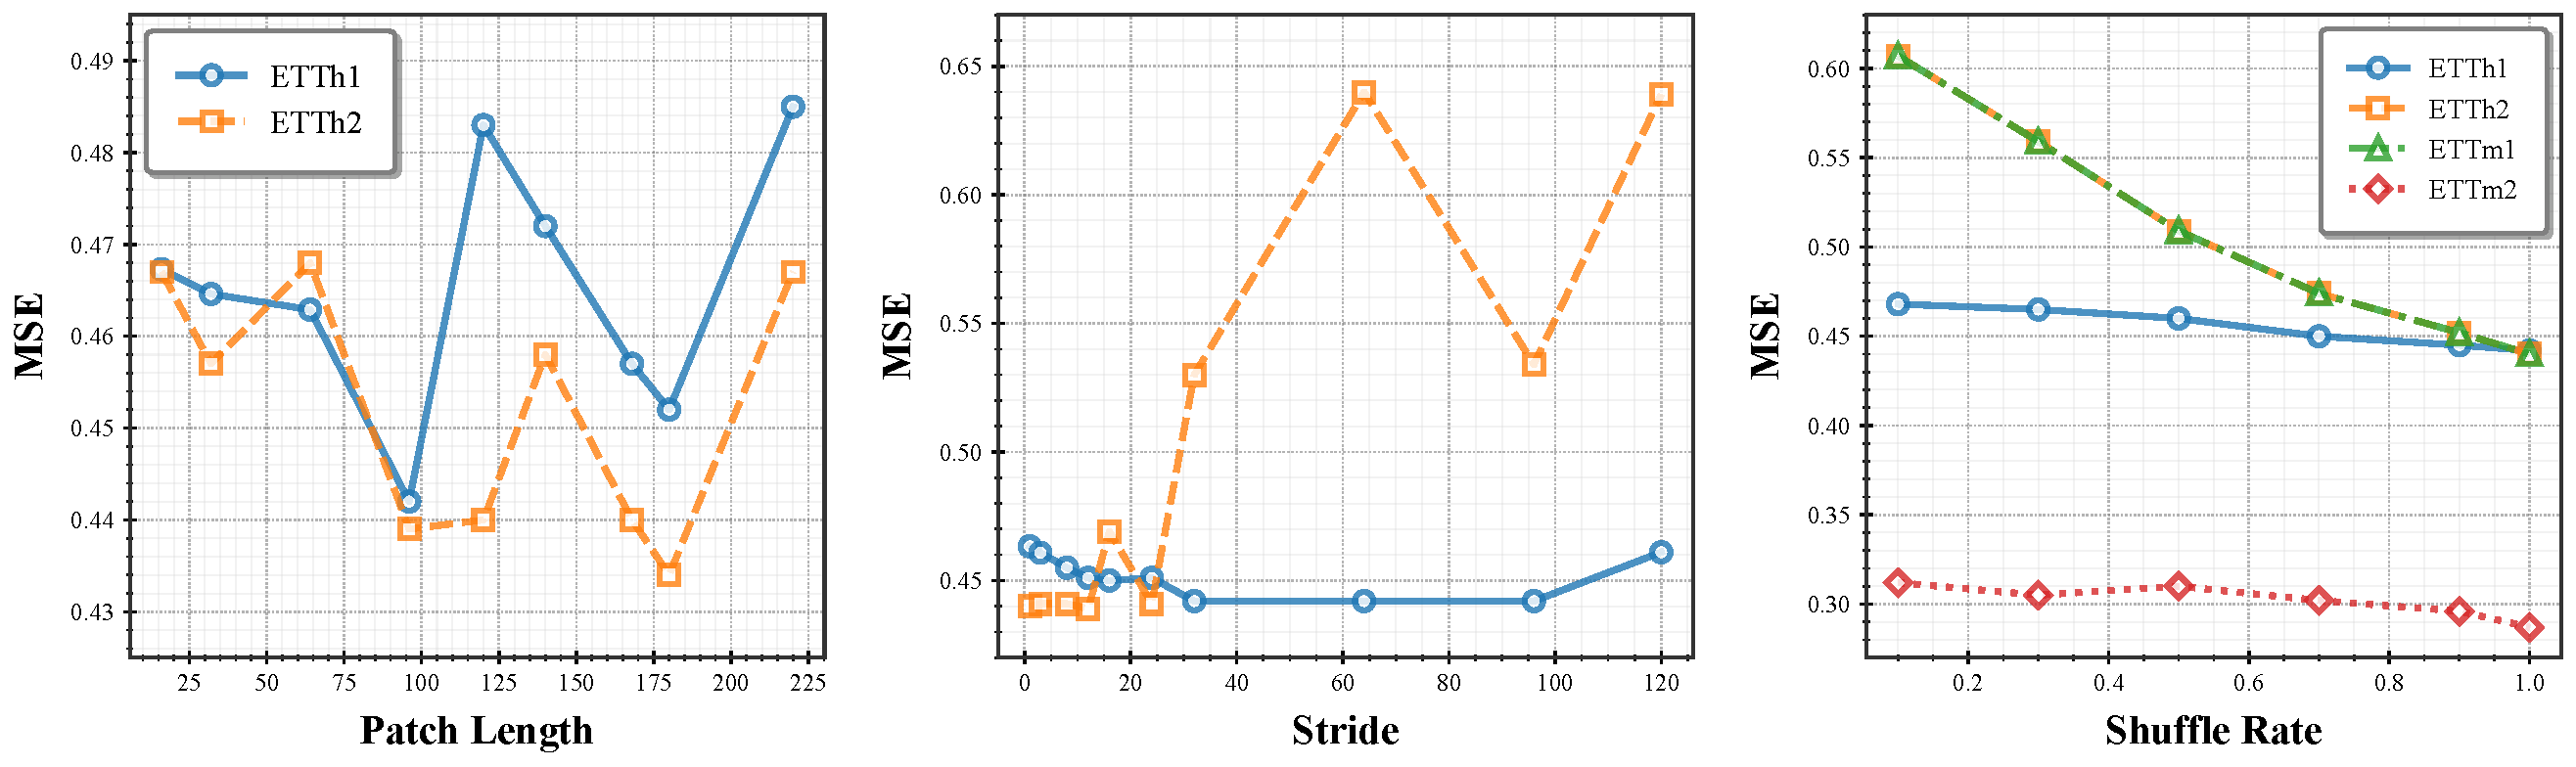
\includegraphics[page=1, width=1.0\textwidth, keepaspectratio]{./images/ablation_study_colorful.pdf}
\caption{Ablation study on the hyperparameter sensitivity of the TPS method. The y-axis shows the MSE averaged over five runs, while the x-axis represents the patch length, stride, or shuffle rate. Experiments were conducted using the LightTS model with a prediction length of 336 on the ETT datasets.}
    \label{fig:ablation_lightts}
\end{figure}


Following the evaluation protocol outlined in the paper~\cite{zhao2024dominantshufflesimplepowerful}, we conducted experiments using t-distributed stochastic neighbor embeddings (t-SNE) to compare the original data and the augmented data generated by each augmentation method on the ETTh2 dataset, utilizing the DLinear model with a prediction length of 336 (see Figure~\ref{fig:tsne}). We applied various augmentation techniques, including Upsample, FreqAdd, FreqPool, FreqMask, FreqMix, Dominant Shuffle, and our proposed method, TPS, with different parameter settings. The TPS parameters—denoted as (patch length, stride, shuffle rate)—were carefully tuned, and the configuration (32, 5, 1) yielded the best performance for the ETTh2 dataset. Our analysis suggests that ETTh2 does not require heavy noise injection, which aligns with the choice of smaller patch and stride values. TPS enables the generation of diverse augmented samples while preserving the core characteristics of the original signal, thereby showcasing the method's flexibility through parameter tuning. For instance, using a different configuration such as (120, 24, 1) introduces more noise due to larger patching, yet it still maintains the underlying signal structure, highlighting TPS's robustness across different augmentation intensities.



\begin{figure}[h!]
    \centering
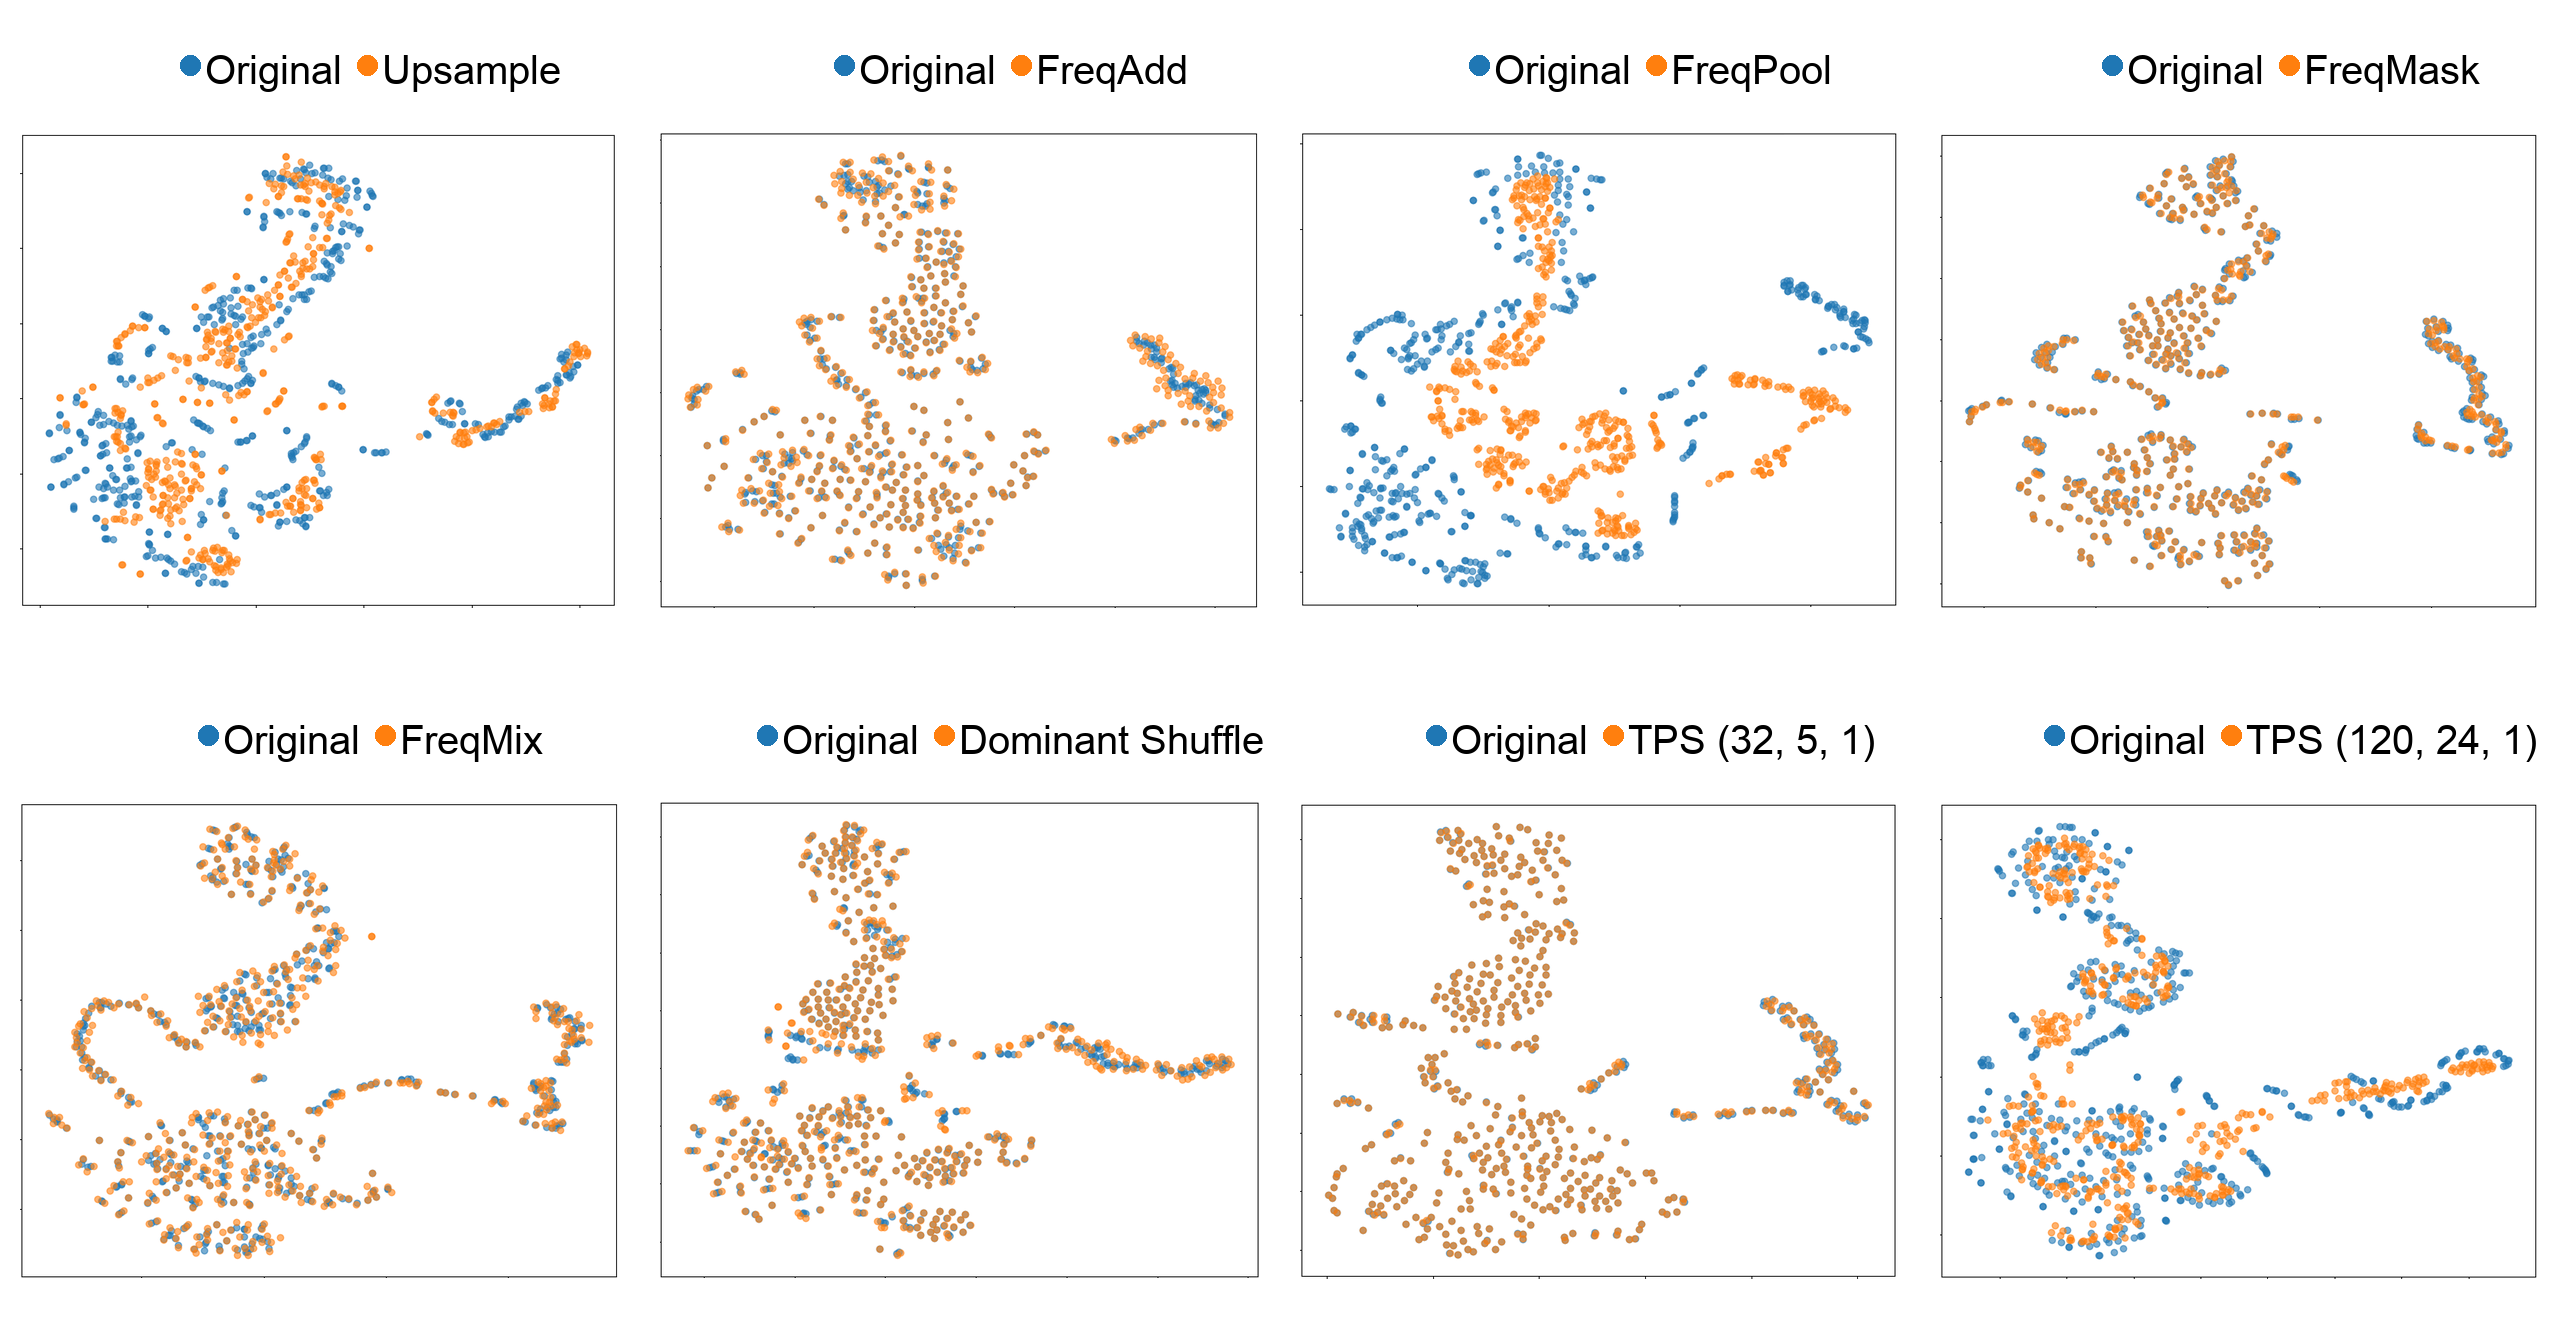
\includegraphics[page=1, width=1.0\textwidth, keepaspectratio]{./images/tsne_result.png}
\caption{t-SNE visualization of original and augmented data on the ETTh2 dataset using the DLinear model with a prediction length of 336.  A closer overlap between the original and augmented points indicates better distributional alignment and lower out-of-distribution issue. \textbf{Best viewed in color.}}
    \label{fig:tsne}
\end{figure}




To quantitatively assess the distributional similarity, we computed three metrics:
\begin{itemize}
    \item The \textbf{Kolmogorov–Smirnov (KS) statistic} measures the maximum difference between the cumulative distribution functions of two data, with higher values indicating greater distributional divergence~\cite{gchron-5-263-2023}.

    \item The \textbf{Wasserstein Distance}, which quantifies the minimum effort required to transform one distribution into another, is more robust to differences in shape than the KS statistic~\cite{gchron-5-263-2023, Iglesias2023}.
    
    \item The \textbf{Dynamic Time Warping (DTW)} distance, commonly used for time series, measures similarity between sequences~\cite{iwana2020timeseriesdataaugmentation, Iglesias2023}.


\end{itemize}

As shown in Table~\ref{tab:dist_metrics}, TPS (32, 5, 1) demonstrates superior performance across the most critical metrics, achieving the lowest Wasserstein distance (0.0097) and DTW distance (1.46), indicating exceptional preservation of both distributional geometry and temporal structure. While the KS statistic (0.0848) is moderate compared to Dominant Shuffle (0.0688), this suggests that TPS introduces controlled distributional variations without destroying fundamental data characteristics. The dramatically lower DTW distance for TPS compared to other methods (1.46 vs. 4.91-14.72) highlights its superior ability to maintain temporal dependencies, which are crucial for forecasting tasks. These results support our hypothesis that TPS generates realistic and semantically consistent augmentations with minimal distributional shift, successfully balancing the trade-off between introducing beneficial variations and preserving essential time series characteristics.

\begin{table}[h!]
\centering
\renewcommand{\arraystretch}{1.0}
\begin{adjustbox}{max width=\textwidth}
\begin{tabular}{lccc}
\toprule
\textbf{Method} & \textbf{Avg. KS Stat} $\downarrow$ & \textbf{Avg. Wasserstein} $\downarrow$ & \textbf{Avg. DTW} $\downarrow$ \\
\midrule
Upsample            & 0.0202 & 0.0177 & 8.73 \\
FreqAdd             & 0.1019 & 0.1475 & 8.55 \\
FreqPool            & 0.3366 & 0.3839 & 14.72 \\
FreqMask            & 0.0793 & 0.0523 & 4.91 \\
FreqMix             & 0.0756 & 0.0855 & 7.12 \\
Dominant Shuffle    & \textbf{0.0688} & 0.0550 & 6.02 \\
TPS (32, 5, 1)      & 0.0848 & \textbf{0.0097} & \textbf{1.46} \\
\bottomrule
\end{tabular}
\end{adjustbox}
\caption{Comparison of distribution shift metrics across various augmentation methods on the ETTh2 dataset using the DLinear model with a prediction length of 336. The metrics include the average Kolmogorov–Smirnov (KS) statistic, Wasserstein distance, and Dynamic Time Warping (DTW), where lower values indicate greater similarity to the original data.}
\label{tab:dist_metrics}
\end{table}


The ablation study in Figure~\ref{fig:augsizetsf} describes experiments conducted with varying augmentation sizes—1, 2, 3, 4, and 5—using the PatchTST model on the ETTh1 and ETTh2 datasets with a prediction length of 96. An augmentation size of 2 means that the augmented sample set is doubled by applying the augmentation method twice. This analysis helps to determine whether each method continues to improve performance as the augmentation size increases or whether it introduces excessive external noise.
The results show that FreqMix benefits from increased augmentation size on both datasets and FreqMask improves only on ETTh2 when applied twice. In contrast, other methods tend to degrade in performance as augmentation size increases. Notably, TPS on ETTh1 shows minimal performance variation even at an augmentation size of 4, suggesting that it introduces little external noise. This is not the case for methods like Upsample and FreqMask, which show greater sensitivity.
Dominant Shuffle and FreqMix exhibit stable performance across augmentation sizes and appear not to introduce significant noise. On the ETTh2 dataset, however, TPS shows signs of performance degradation at higher augmentation sizes, possibly due to suboptimal hyperparameter settings. Nonetheless, for other models and prediction lengths on ETTh2, TPS has shown to be generally stable across different augmentation sizes.


\begin{figure}[h!]
    \centering
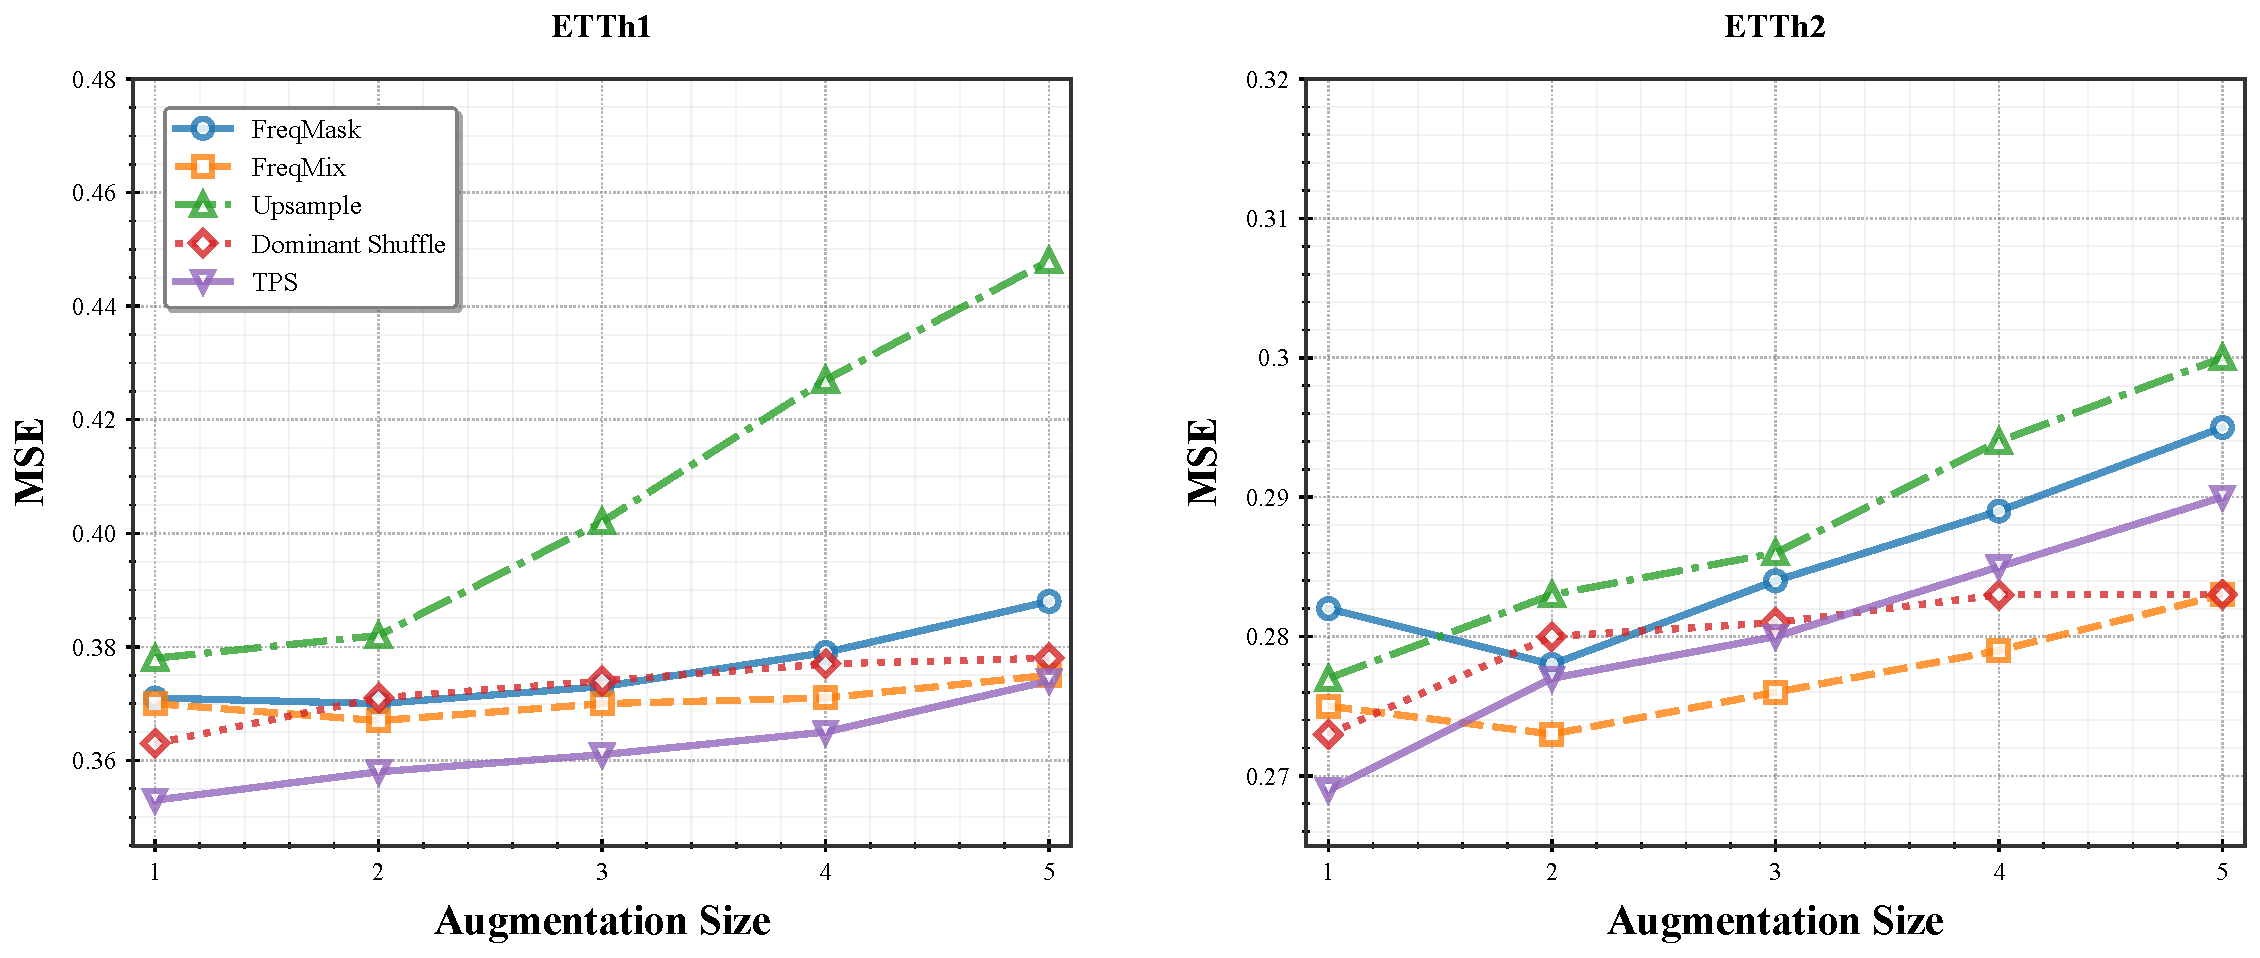
\includegraphics[page=1, width=1.0\textwidth, keepaspectratio]{./images/augmentation_size_analysis.pdf}
\caption{Impact of varying augmentation sizes (1–5) on forecasting performance using the PatchTST model with a prediction length of 96 on the ETTh1 and ETTh2 datasets. The results demonstrate how different augmentation methods respond to increasing augmentation intensity, highlighting stability or degradation in performance.}
    \label{fig:augsizetsf}
\end{figure}





We conducted experiments using different augmentation ratios — 0.1, 0.3, 0.5, 0.7, and 1.0 — with the PatchTST model on the ETTh1 and ETTh2 datasets, using a prediction length of 96 in the Figure~\ref{fig:augratio}. The augmentation methods evaluated include FreqMask, FreqMix, Upsample, Dominant Shuffle, and our proposed method, TPS. Here, the augmentation ratio refers to the proportion of augmented samples included in each training batch, meaning that lower ratios correspond to fewer augmented samples.

Our results show that TPS consistently achieves the lowest MSE across both datasets when using the full augmentation ratio (1.0). Remarkably, even with only 10\% (i.e., a ratio of 0.1) of augmented samples, TPS outperforms all other augmentation methods at their respective ratios.

\begin{figure}[h!]
    \centering
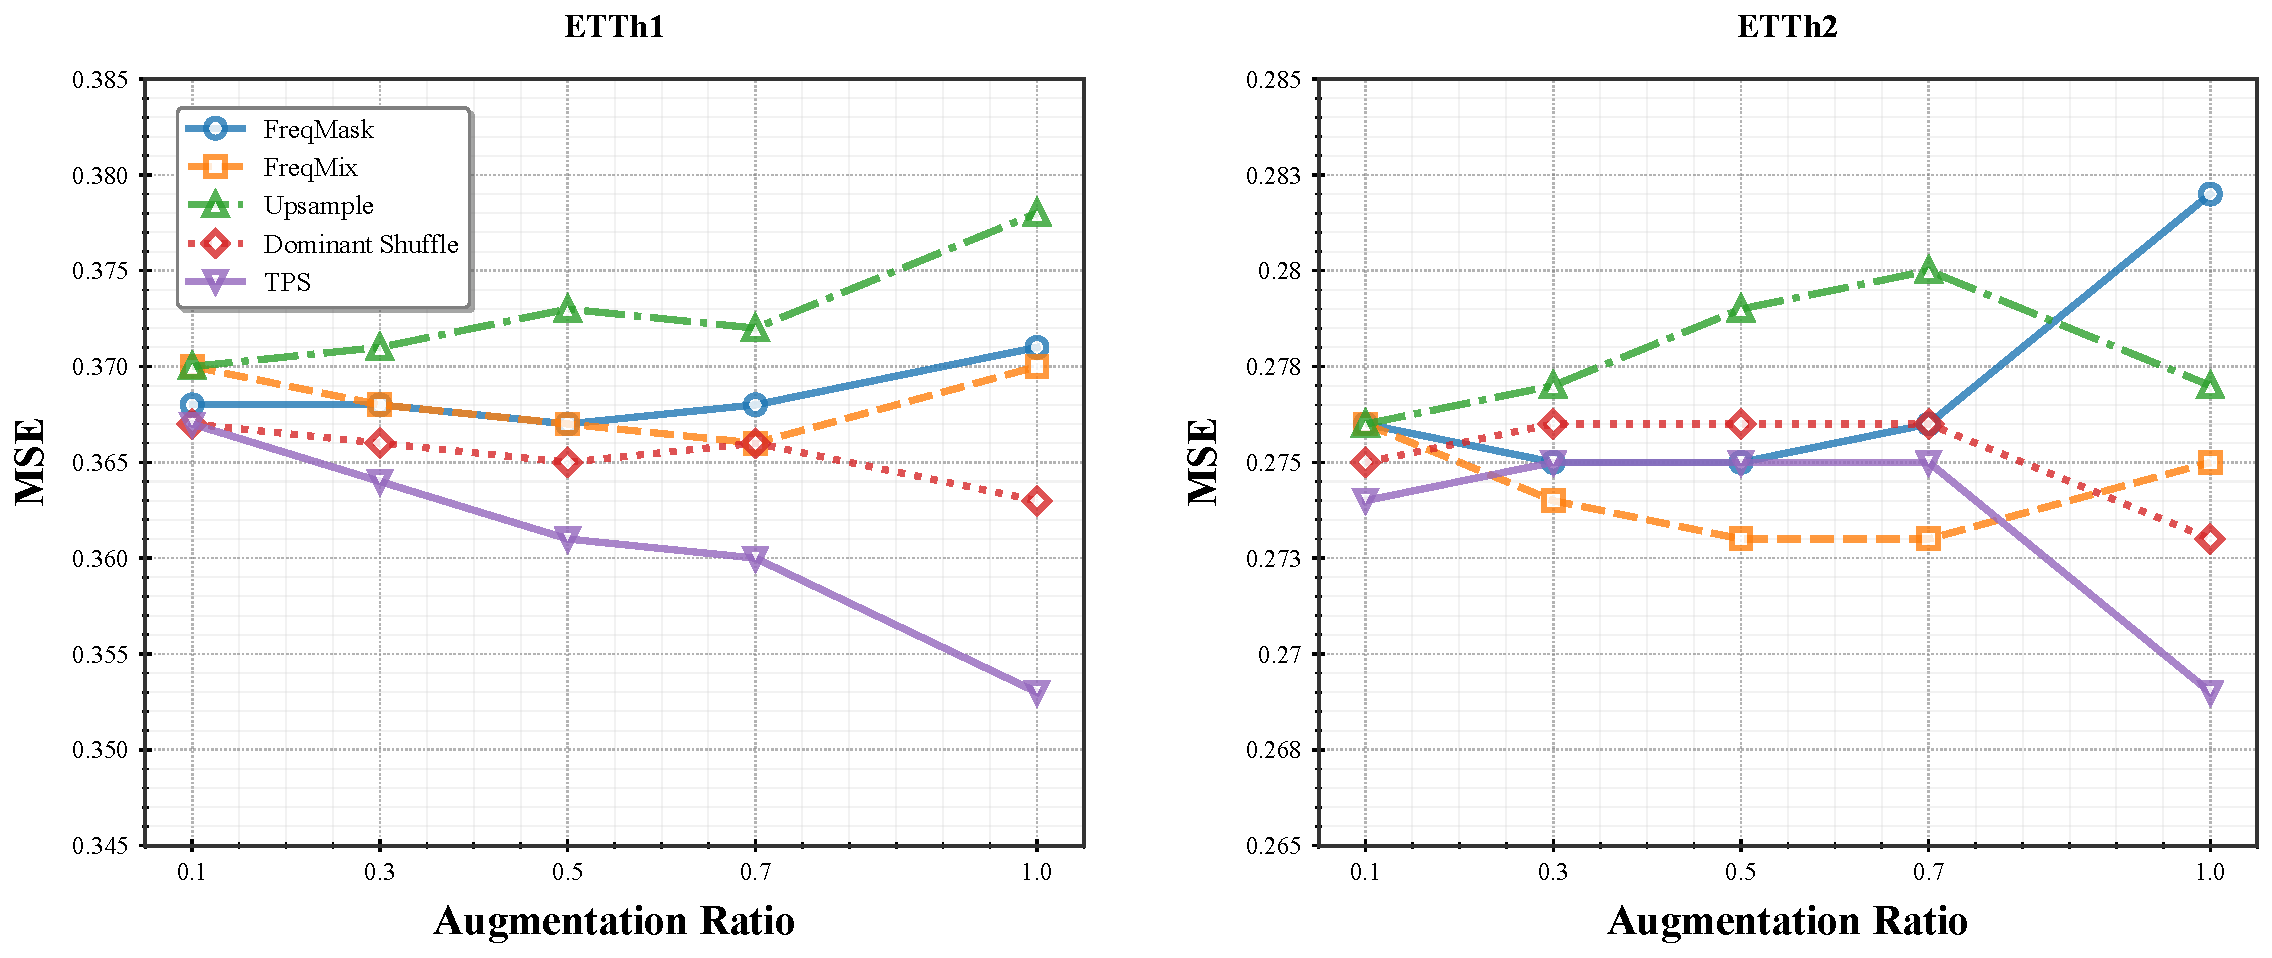
\includegraphics[page=1, width=1.0\textwidth, keepaspectratio]{./images/augmentation_ratio_analysis.pdf}
\caption{Effect of varying augmentation ratios (0.1 to 1.0) on the MSE performance of different augmentation methods using the PatchTST model with prediction length 96 on the ETTh1 and ETTh2 datasets. The augmentation ratio indicates the proportion of augmented samples used during training.}
    \label{fig:augratio}
\end{figure}



The final ablation study for time series forecasting evaluates the impact of different data augmentation methods on training time. Table~\ref{tab:augmentation_comparison} summarizes this comparison, conducted using the TSMixer model on the ETTh2 dataset with a prediction length of 720. The \textbf{Aug. Time} column reports the time required to apply the augmentation (in milliseconds), while the \textbf{Epoch Time} indicates the average training time per epoch (in seconds). The \textbf{Overhead} column shows the relative increase in epoch time (\%) compared to the baseline with no augmentation.

As shown in the table, TPS introduces a moderate augmentation time and only a modest increase in epoch time relative to the baseline. In contrast, Dominant Shuffle significantly increases the training cost, more than tripling the epoch time. Notably, for most augmentation methods (including TPS), the overhead remains well below twice the baseline training time. For Dominant Shuffle, we used the authors’ original implementation.


\begin{table}[h!]
\centering
\footnotesize
\vspace{0.2cm}
\renewcommand{\arraystretch}{1.1}
\begin{tabular}{lccc}
    \toprule
    \textbf{Method} & \textbf{Aug. Time (ms)} & \textbf{Epoch Time (s)} & \textbf{Overhead (\%)} \\
    \midrule
    None  & 0.000 & 2.298 & 0.00 \\
    \midrule
    FreqPool        & 1.023 & 2.611 & 13.63 \\
    FreqMask        & 1.097 & 2.633 & 14.59 \\
    FreqAdd         & 1.151 & 2.635 & 14.67 \\
    RobustTAD-m     & 1.603 & 2.690 & 17.08 \\
    FreqMix         & 1.573 & 2.720 & 18.36 \\
    RobustTAD-p     & 1.659 & 2.762 & 20.19 \\
    WaveMix         & 2.287 & 2.864 & 24.64 \\
    Upsample        & 2.486 & 2.944 & 28.14 \\
    WaveMask        & 3.809 & 3.145 & 36.86 \\
    \midrule
    TPS            & 7.688  & 4.094 & 78.15 \\
    Dominant Shuffle    & 22.908 & 7.698 & 235.02 \\
    \bottomrule
\end{tabular}
\vspace{0.2cm}
\caption{Comparison of data augmentation methods based on their impact on training time and computational overhead. Results are obtained using the TSMixer model on the ETTh2 dataset with a prediction length of 720. \textit{Aug. Time} refers to the time (in milliseconds) required to apply the augmentation, \textit{Epoch Time} represents the average training time per epoch (in seconds), and \textit{Overhead} indicates the percentage increase in epoch time relative to the baseline (None).}
\label{tab:augmentation_comparison}
\end{table}


\subsection{Ablation studies for Time Series Classification}  \label{subsec:ablation-tsc}

In these two ablation studies for time series classification, we used only MiniRocket for the univariate datasets and followed the same training pipeline throughout.

Figure~\ref{fig:augratiotsc} presents the ablation study on augmentation size for classification tasks, conducted on nine univariate time series datasets using the MiniRocket model. For each dataset, we selected the top five augmentation methods and compared them against our proposed method, TIPS, across augmentation sizes ranging from 1 to 5. For example, an augmentation size of 2 means each sample is augmented twice, effectively doubling the size of the augmented data.
From the figure, we observe that—except for the \textit{Car} and \textit{Meat} datasets—TIPS consistently maintains its superior performance across all augmentation sizes of the top five competing methods. In the \textit{Beef} dataset, TIPS improves from third place to second when using two augmentations. Overall, our method achieves its peak accuracy with one or sometimes two augmentation sizes. Beyond this point, additional augmentation does not lead to further improvements, indicating that TIPS is highly effective with minimal augmentation size. In contrast, some other methods often require four augmented samples to reach their maximum performance.


\begin{figure}[h!]
    \centering
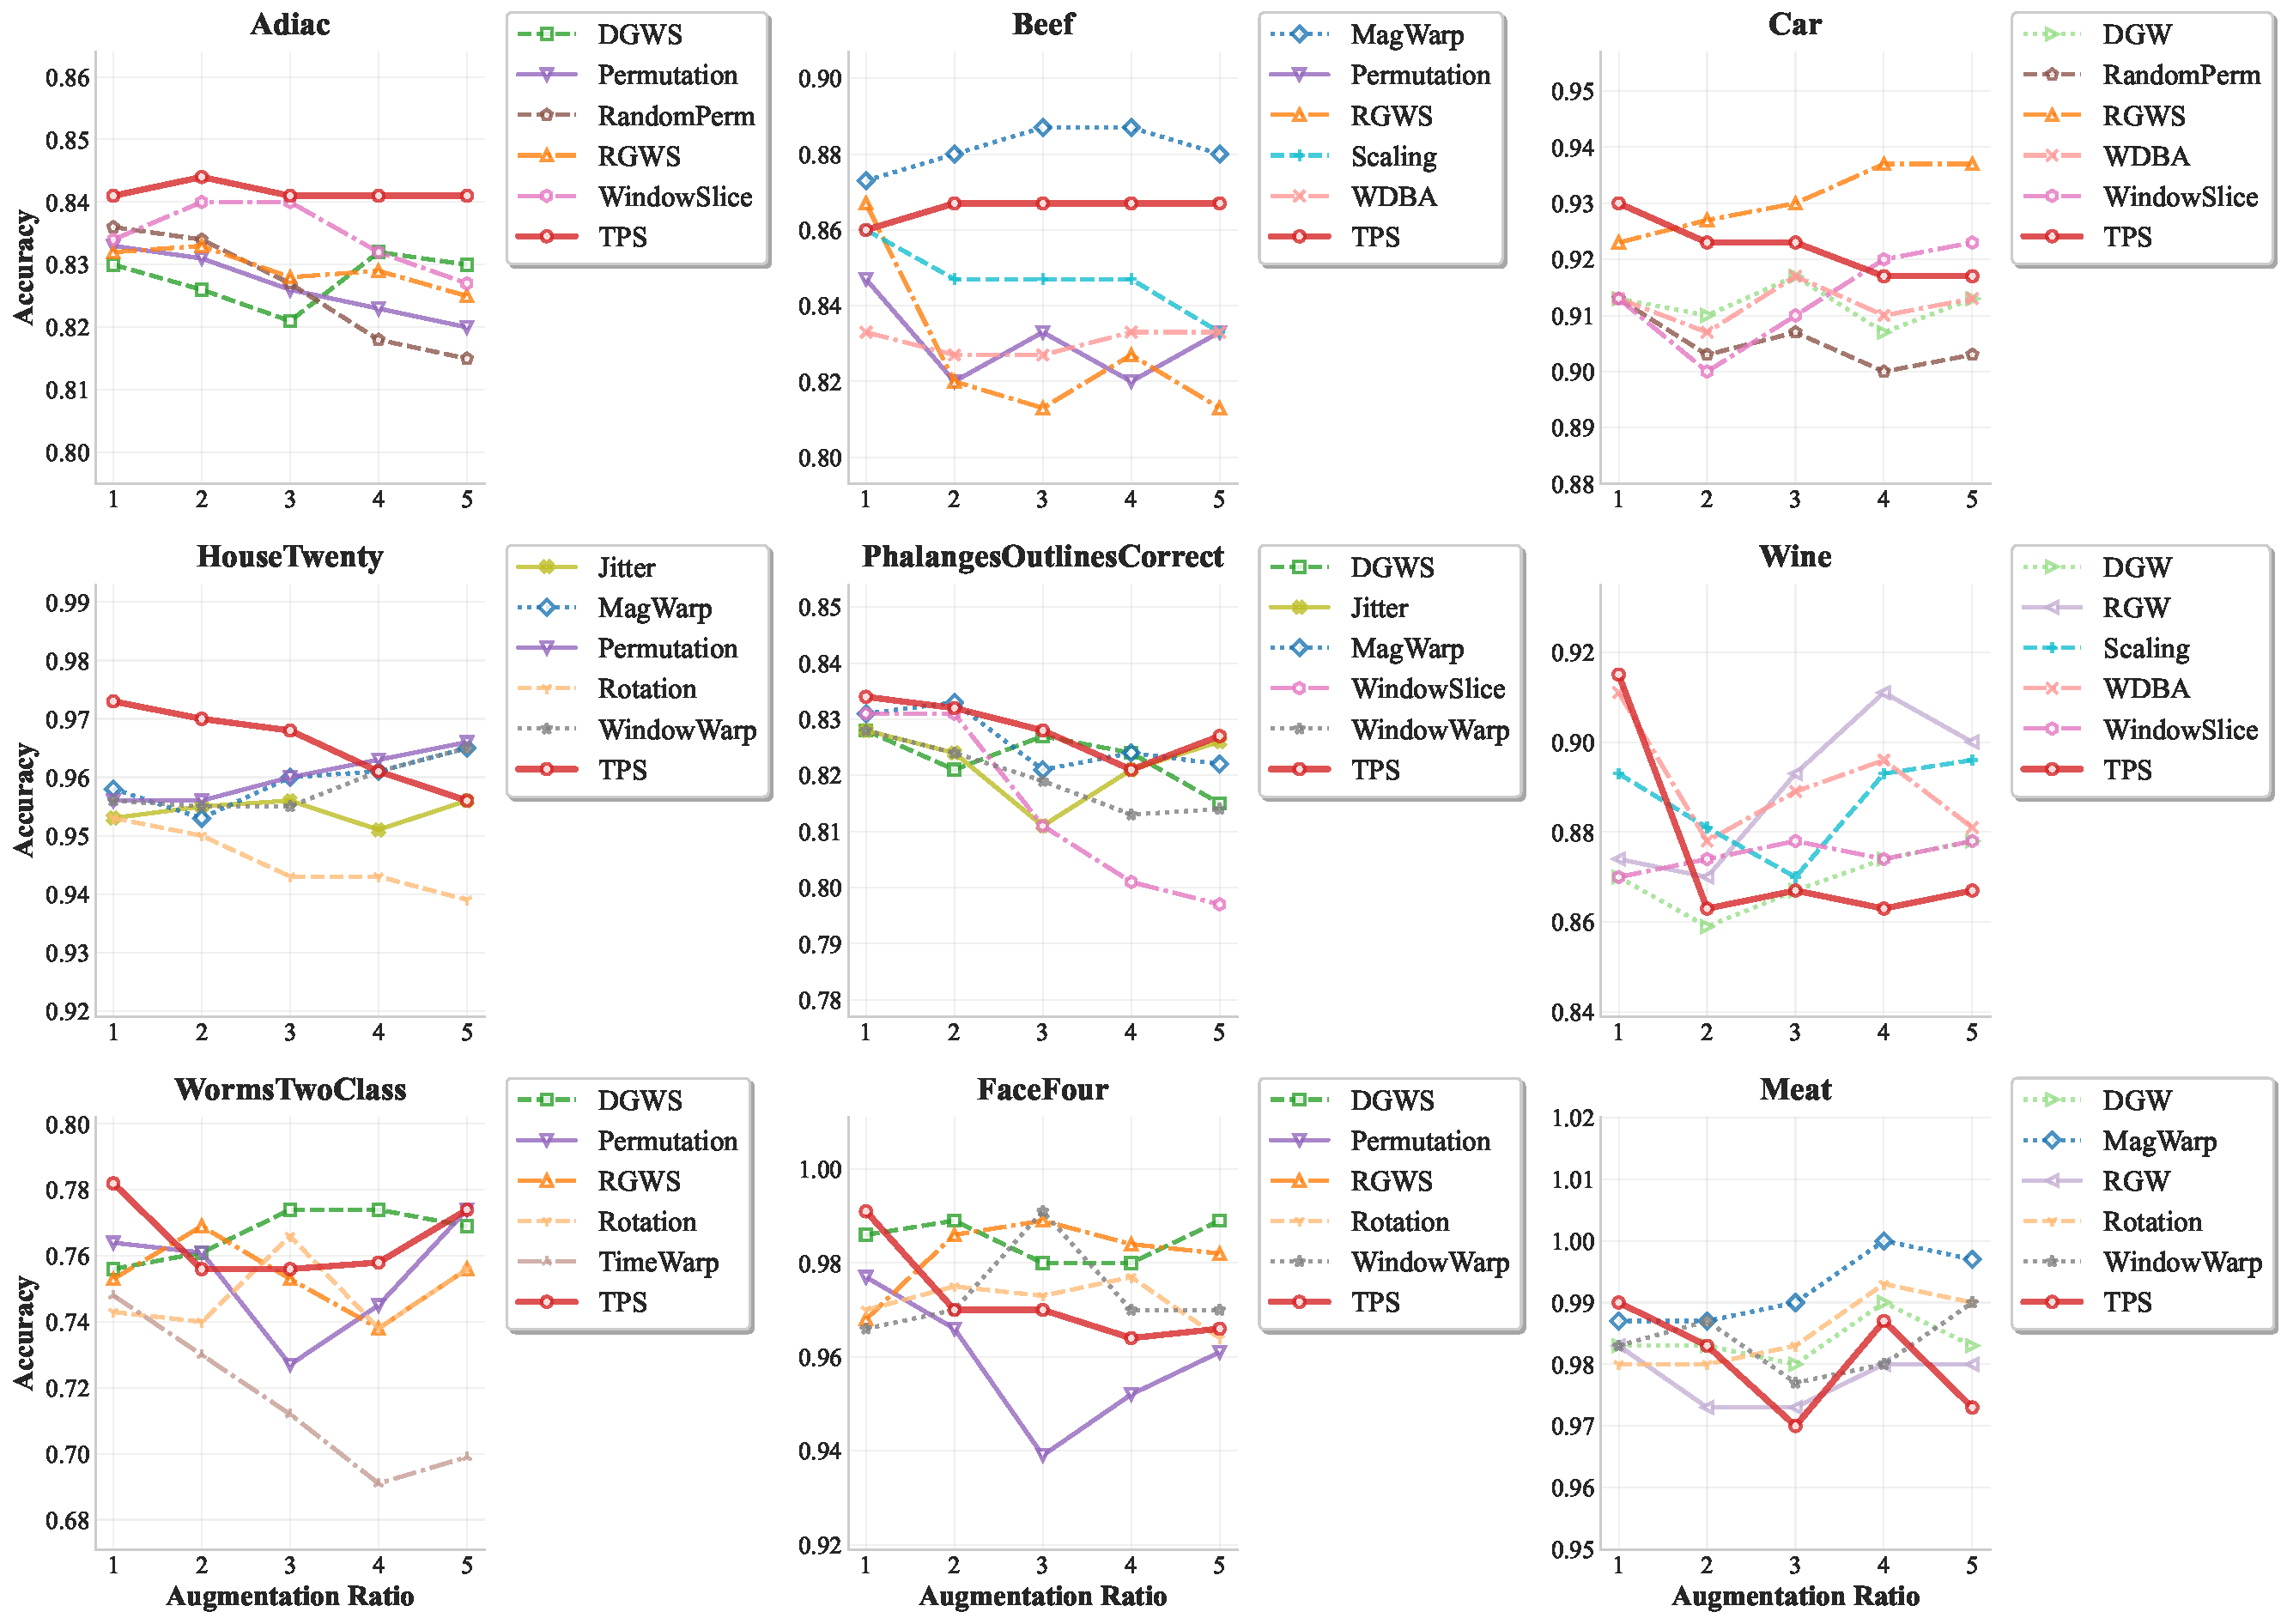
\includegraphics[page=1, width=1.0\textwidth, keepaspectratio]{./images/improved_tsc_results.pdf}
\caption{Ablation study on augmentation size for classification tasks across 9 univariate time series datasets using MiniRocket. For each dataset, the top five augmentation methods are compared against our proposed method TIPS. Augmentation sizes from 1 to 5 are evaluated.}
    \label{fig:augratiotsc}
\end{figure}




The final ablation study for classification tasks examines the runtime of each augmentation method. Table~\ref{tab:aug_times_tsc} reports the time required to execute each method, measured in seconds under the MiniRocket model on the HandOutlines dataset. The \textbf{Aug. Time} column indicates the time taken by each augmentation.
We observe that TIPS has a moderate runtime compared to other fast augmentations, such as Magnitude Warping and Time Warping; however, it is significantly more efficient than computationally intensive methods like RGW and DGW. This highlights that our method achieves superior classification performance with substantially lower computational cost than the most complex augmentation strategies.

\begin{table}[h!]
\centering
\begin{tabular}{lr}
\toprule
\textbf{Method} & \textbf{Aug. Time (s)} \\
\midrule
 Jitter         & 0.14 \\
 Scaling        & 0.04 \\
 Rotation       & 0.04 \\
 Permutation    & 0.08 \\
 RandPermutation   & 0.13 \\
 Mag. Warping        & 0.45 \\
 Time Warping       & 0.52 \\
 Window Slice    & 0.12 \\
 Window Warping     & 0.17 \\
 TIPS           & 49.76 \\
SPAWNER        & 1,612.38 \\
RGW            & 1,761.13 \\
RGWs           & 15,334.64 \\
 DGW            & 26,287.65 \\
 wDBA           & 59,832.97 \\
 DGWs           & 247,505.86 \\
\bottomrule
\end{tabular}
\caption{Runtime (in seconds) for various time series augmentation methods on the HandOutlines dataset using the MiniRocket model. The results reflect the computational cost required to apply each augmentation.}

\label{tab:aug_times_tsc}
\end{table}






